\documentclass[9pt]{article}

\PassOptionsToPackage{hyphens}{url}\usepackage{hyperref}

\setlength{\parindent}{20pt}
\setlength{\parskip}{5pt}

\usepackage{xcolor}
\usepackage[english]{babel}
\usepackage{nameref}
\usepackage{footnote}
\usepackage{refcount}
\usepackage{makecell}
\usepackage[a4paper, total={6in, 10in}]{geometry}
\usepackage{titlesec}
\usepackage{graphicx}
\usepackage{setspace}
\usepackage{url}
\usepackage{amsmath,amsfonts,amssymb}
%\usepackage{indentfirst}
\usepackage{float}
\usepackage{pgf}
\usepackage{color,soul}
\usepackage{tabularx}	

\makesavenoteenv{tabular}
\makesavenoteenv{table}

\setcounter{secnumdepth}{5}
\setcounter{tocdepth}{4}

\titleformat{\paragraph}
{\normalfont\normalsize\bfseries}{\theparagraph}{1em}{}
\titlespacing*{\paragraph}
{0pt}{3.25ex plus 1ex minus .2ex}{1.5ex plus .2ex}

\usepackage[bottom]{footmisc}

\DeclareUnicodeCharacter{2212}{-}

\newcommand\inputpgf[2]{{
\let\pgfimageWithoutPath\pgfimage
\renewcommand{\pgfimage}[2][]{\pgfimageWithoutPath[##1]{#1/##2}}
\input{#1/#2}
}}

% table col separation
\setlength\tabcolsep{0pt}


% -------------------- %
% Start document %
% -------------------- %
\begin{document}

	% -------------------- %
	% Python content %
	% -------------------- %
	
\section{Misclassified images}


        In the following 90 images are listed, which are not correctly classified in
        the top-1 or top-5 classification.
    \\

\raggedright
\begin{tabularx}{\textwidth}{X r}
    \textbf{Used dataset} & \texttt{raw-train/food-50-80-20-all}\\
    \textbf{Experiment} & \texttt{food-50-80-20-without-data-augmentation}
\end{tabularx}

\raggedright
\vspace{6pt}
\begin{tabularx}{\textwidth}{X r}
    \textbf{Number of trained files} & 49.943\\
    \textbf{Number of validated files} & 2.953
\end{tabularx}

\raggedright
\vspace{6pt}
\begin{tabularx}{\textwidth}{X r}
    \textbf{Used CNN model} & InceptionV3\\
    \textbf{Used weights (transfer learning)} & Imagenet
\end{tabularx}

\raggedright
\vspace{6pt}
\begin{tabularx}{\textwidth}{X r}
    \textbf{Accuracy} & 83.59 \%\\
    \textbf{Best epoch} & 21
\end{tabularx}
    
\subsection{Baked Beans}
    
\subsubsection{baked\textunderscore beans/baked-beans116.png}

\begin{minipage}[t]{0.4\textwidth}
	\vspace{0pt}
	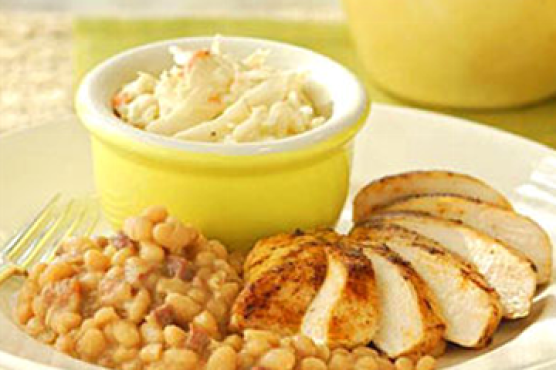
\includegraphics[width=\linewidth]{images/evaluation-images/baked_beans/baked-beans116.png}
\end{minipage}
\hfill
\begin{minipage}[t]{0.5\textwidth}
	\vspace{0pt}\raggedright
	\begin{tabularx}{\textwidth}{X r}
		\small \textbf{Real class} & \small Baked Beans\\
		\small \textbf{Predicted class} & \small Bundt Cake\\
		\small \textbf{Predicted accuracy} & \small 18.41 \%
    \end{tabularx}\\
    
    \vspace{6pt}
	\begin{tabularx}{\textwidth}{X r}
        \small \textbf{Top-5} & \small \textbf{Accuracy} \\
        \hline
		\small 1) Bundt Cake & \small 18.41 \%\\\small 2) Mashed Potatoes & \small 11.22 \%\\\small 3) Pancakes & \small 11.13 \%\\\small 4) Cinnamon Roll & \small 7.41 \%\\\small 5) Ice Cream & \small 7.36 \%
    \end{tabularx}
\end{minipage}
    
\subsubsection{baked\textunderscore beans/baked-beans89.jpeg}

\begin{minipage}[t]{0.4\textwidth}
	\vspace{0pt}
	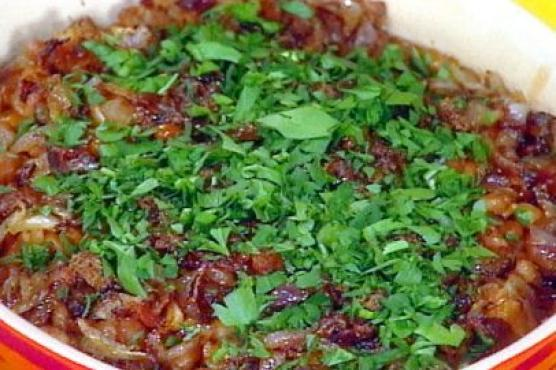
\includegraphics[width=\linewidth]{images/evaluation-images/baked_beans/baked-beans89.jpeg}
\end{minipage}
\hfill
\begin{minipage}[t]{0.5\textwidth}
	\vspace{0pt}\raggedright
	\begin{tabularx}{\textwidth}{X r}
		\small \textbf{Real class} & \small Baked Beans\\
		\small \textbf{Predicted class} & \small Nachos\\
		\small \textbf{Predicted accuracy} & \small 36.67 \%
    \end{tabularx}\\
    
    \vspace{6pt}
	\begin{tabularx}{\textwidth}{X r}
        \small \textbf{Top-5} & \small \textbf{Accuracy} \\
        \hline
		\small 1) Nachos & \small 36.67 \%\\\small 2) Salad & \small 21.63 \%\\\small 3) Pizza & \small 7.29 \%\\\small 4) Beef Stew & \small 5.15 \%\\\small 5) Cobb Salad & \small 4.47 \%
    \end{tabularx}
\end{minipage}
    
\subsection{Baked Salmon}
    
\subsubsection{baked\textunderscore salmon/baked-salmon11.jpg}

\begin{minipage}[t]{0.4\textwidth}
	\vspace{0pt}
	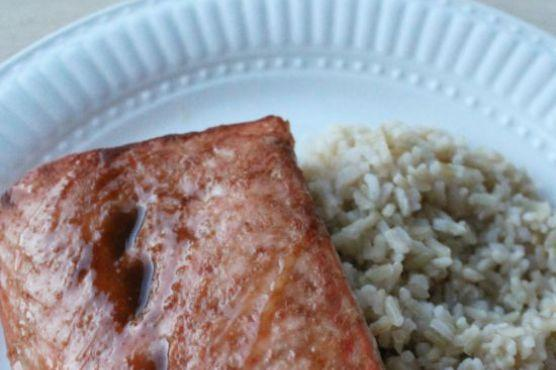
\includegraphics[width=\linewidth]{images/evaluation-images/baked_salmon/baked-salmon11.jpg}
\end{minipage}
\hfill
\begin{minipage}[t]{0.5\textwidth}
	\vspace{0pt}\raggedright
	\begin{tabularx}{\textwidth}{X r}
		\small \textbf{Real class} & \small Baked Salmon\\
		\small \textbf{Predicted class} & \small Meatloaf\\
		\small \textbf{Predicted accuracy} & \small 26.88 \%
    \end{tabularx}\\
    
    \vspace{6pt}
	\begin{tabularx}{\textwidth}{X r}
        \small \textbf{Top-5} & \small \textbf{Accuracy} \\
        \hline
		\small 1) Meatloaf & \small 26.88 \%\\\small 2) Calzone & \small 26.17 \%\\\small 3) Pizza & \small 7.34 \%\\\small 4) Empanada & \small 6.14 \%\\\small 5) Lasagne & \small 5.05 \%
    \end{tabularx}
\end{minipage}
    
\subsubsection{baked\textunderscore salmon/baked-salmon14.jpg}

\begin{minipage}[t]{0.4\textwidth}
	\vspace{0pt}
	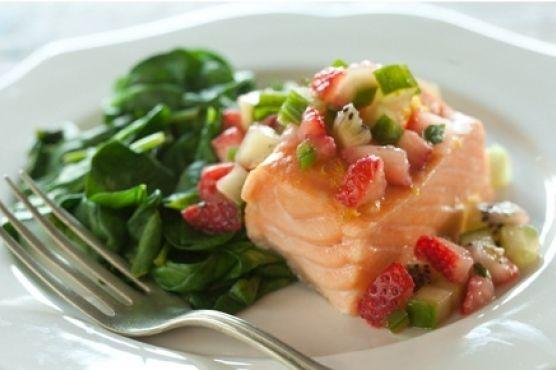
\includegraphics[width=\linewidth]{images/evaluation-images/baked_salmon/baked-salmon14.jpg}
\end{minipage}
\hfill
\begin{minipage}[t]{0.5\textwidth}
	\vspace{0pt}\raggedright
	\begin{tabularx}{\textwidth}{X r}
		\small \textbf{Real class} & \small Baked Salmon\\
		\small \textbf{Predicted class} & \small Salad\\
		\small \textbf{Predicted accuracy} & \small 66.80 \%
    \end{tabularx}\\
    
    \vspace{6pt}
	\begin{tabularx}{\textwidth}{X r}
        \small \textbf{Top-5} & \small \textbf{Accuracy} \\
        \hline
		\small 1) Salad & \small 66.80 \%\\\small 2) Macaroni And Cheese & \small 21.98 \%\\\small 3) Nachos & \small 6.23 \%\\\small 4) Omelet & \small 3.57 \%\\\small 5) Cobb Salad & \small 0.33 \%
    \end{tabularx}
\end{minipage}
    
\subsubsection{baked\textunderscore salmon/baked-salmon34.jpg}

\begin{minipage}[t]{0.4\textwidth}
	\vspace{0pt}
	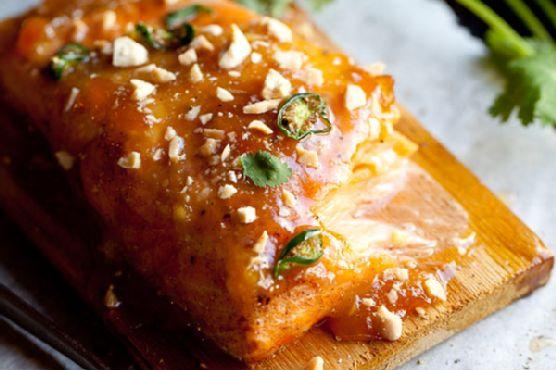
\includegraphics[width=\linewidth]{images/evaluation-images/baked_salmon/baked-salmon34.jpg}
\end{minipage}
\hfill
\begin{minipage}[t]{0.5\textwidth}
	\vspace{0pt}\raggedright
	\begin{tabularx}{\textwidth}{X r}
		\small \textbf{Real class} & \small Baked Salmon\\
		\small \textbf{Predicted class} & \small Pizza\\
		\small \textbf{Predicted accuracy} & \small 99.61 \%
    \end{tabularx}\\
    
    \vspace{6pt}
	\begin{tabularx}{\textwidth}{X r}
        \small \textbf{Top-5} & \small \textbf{Accuracy} \\
        \hline
		\small 1) Pizza & \small 99.61 \%\\\small 2) Calzone & \small 0.13 \%\\\small 3) Lasagne & \small 0.11 \%\\\small 4) Meatloaf & \small 0.08 \%\\\small 5) Burrito & \small 0.01 \%
    \end{tabularx}
\end{minipage}
    
\subsubsection{baked\textunderscore salmon/baked-salmon36.jpg}

\begin{minipage}[t]{0.4\textwidth}
	\vspace{0pt}
	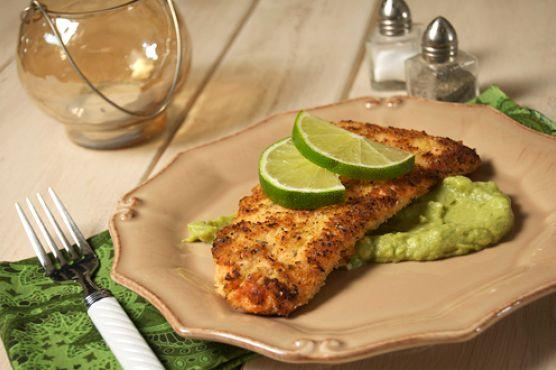
\includegraphics[width=\linewidth]{images/evaluation-images/baked_salmon/baked-salmon36.jpg}
\end{minipage}
\hfill
\begin{minipage}[t]{0.5\textwidth}
	\vspace{0pt}\raggedright
	\begin{tabularx}{\textwidth}{X r}
		\small \textbf{Real class} & \small Baked Salmon\\
		\small \textbf{Predicted class} & \small Chicken Wings\\
		\small \textbf{Predicted accuracy} & \small 48.19 \%
    \end{tabularx}\\
    
    \vspace{6pt}
	\begin{tabularx}{\textwidth}{X r}
        \small \textbf{Top-5} & \small \textbf{Accuracy} \\
        \hline
		\small 1) Chicken Wings & \small 48.19 \%\\\small 2) Grilled Cheese Sandwich & \small 37.19 \%\\\small 3) Kebabs & \small 8.52 \%\\\small 4) Quesadilla & \small 1.22 \%\\\small 5) Chicken Piccata & \small 1.01 \%
    \end{tabularx}
\end{minipage}
    
\subsubsection{baked\textunderscore salmon/baked-salmon37.jpg}

\begin{minipage}[t]{0.4\textwidth}
	\vspace{0pt}
	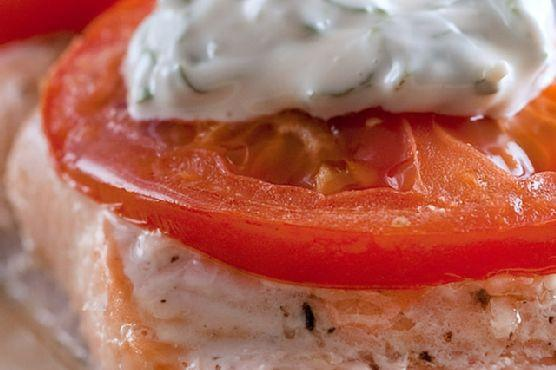
\includegraphics[width=\linewidth]{images/evaluation-images/baked_salmon/baked-salmon37.jpg}
\end{minipage}
\hfill
\begin{minipage}[t]{0.5\textwidth}
	\vspace{0pt}\raggedright
	\begin{tabularx}{\textwidth}{X r}
		\small \textbf{Real class} & \small Baked Salmon\\
		\small \textbf{Predicted class} & \small Burger\\
		\small \textbf{Predicted accuracy} & \small 87.55 \%
    \end{tabularx}\\
    
    \vspace{6pt}
	\begin{tabularx}{\textwidth}{X r}
        \small \textbf{Top-5} & \small \textbf{Accuracy} \\
        \hline
		\small 1) Burger & \small 87.55 \%\\\small 2) Cheesecake & \small 4.08 \%\\\small 3) Stuffed Pepper & \small 3.16 \%\\\small 4) Donut & \small 1.05 \%\\\small 5) Cinnamon Roll & \small 0.94 \%
    \end{tabularx}
\end{minipage}
    
\subsubsection{baked\textunderscore salmon/baked-salmon8.jpg}

\begin{minipage}[t]{0.4\textwidth}
	\vspace{0pt}
	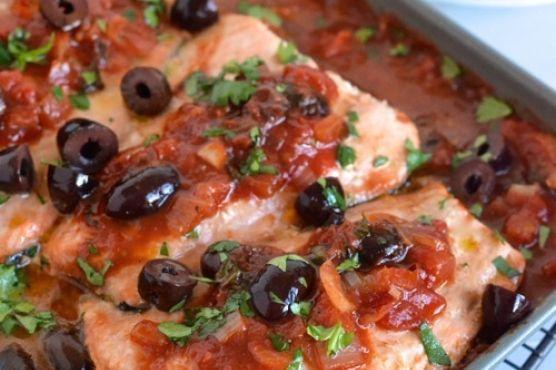
\includegraphics[width=\linewidth]{images/evaluation-images/baked_salmon/baked-salmon8.jpg}
\end{minipage}
\hfill
\begin{minipage}[t]{0.5\textwidth}
	\vspace{0pt}\raggedright
	\begin{tabularx}{\textwidth}{X r}
		\small \textbf{Real class} & \small Baked Salmon\\
		\small \textbf{Predicted class} & \small Pizza\\
		\small \textbf{Predicted accuracy} & \small 71.11 \%
    \end{tabularx}\\
    
    \vspace{6pt}
	\begin{tabularx}{\textwidth}{X r}
        \small \textbf{Top-5} & \small \textbf{Accuracy} \\
        \hline
		\small 1) Pizza & \small 71.11 \%\\\small 2) Nachos & \small 28.77 \%\\\small 3) Omelet & \small 0.04 \%\\\small 4) Pancakes & \small 0.03 \%\\\small 5) Meatballs & \small 0.01 \%
    \end{tabularx}
\end{minipage}
    
\subsection{Beef Stew}
    
\subsubsection{beef\textunderscore stew/beef-stew118.jpg}

\begin{minipage}[t]{0.4\textwidth}
	\vspace{0pt}
	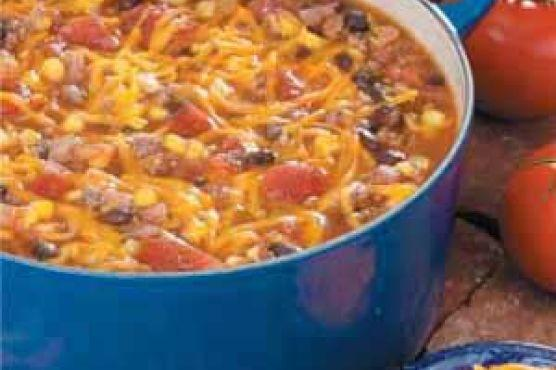
\includegraphics[width=\linewidth]{images/evaluation-images/beef_stew/beef-stew118.jpg}
\end{minipage}
\hfill
\begin{minipage}[t]{0.5\textwidth}
	\vspace{0pt}\raggedright
	\begin{tabularx}{\textwidth}{X r}
		\small \textbf{Real class} & \small Beef Stew\\
		\small \textbf{Predicted class} & \small Macaroni And Cheese\\
		\small \textbf{Predicted accuracy} & \small 60.30 \%
    \end{tabularx}\\
    
    \vspace{6pt}
	\begin{tabularx}{\textwidth}{X r}
        \small \textbf{Top-5} & \small \textbf{Accuracy} \\
        \hline
		\small 1) Macaroni And Cheese & \small 60.30 \%\\\small 2) Baked Beans & \small 15.62 \%\\\small 3) Lasagne & \small 13.69 \%\\\small 4) Spaghetti & \small 3.27 \%\\\small 5) Omelet & \small 1.38 \%
    \end{tabularx}
\end{minipage}
    
\subsubsection{beef\textunderscore stew/beef-stew236.jpg}

\begin{minipage}[t]{0.4\textwidth}
	\vspace{0pt}
	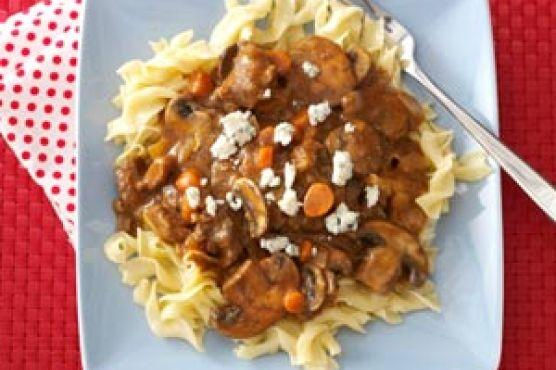
\includegraphics[width=\linewidth]{images/evaluation-images/beef_stew/beef-stew236.jpg}
\end{minipage}
\hfill
\begin{minipage}[t]{0.5\textwidth}
	\vspace{0pt}\raggedright
	\begin{tabularx}{\textwidth}{X r}
		\small \textbf{Real class} & \small Beef Stew\\
		\small \textbf{Predicted class} & \small Beef Stroganoff\\
		\small \textbf{Predicted accuracy} & \small 94.96 \%
    \end{tabularx}\\
    
    \vspace{6pt}
	\begin{tabularx}{\textwidth}{X r}
        \small \textbf{Top-5} & \small \textbf{Accuracy} \\
        \hline
		\small 1) Beef Stroganoff & \small 94.96 \%\\\small 2) Meatballs & \small 4.18 \%\\\small 3) Spaghetti & \small 0.45 \%\\\small 4) Macaroni And Cheese & \small 0.17 \%\\\small 5) Nachos & \small 0.13 \%
    \end{tabularx}
\end{minipage}
    
\subsection{Beef Stroganoff}
    
\subsubsection{beef\textunderscore stroganoff/beef-stroganoff122.jpg}

\begin{minipage}[t]{0.4\textwidth}
	\vspace{0pt}
	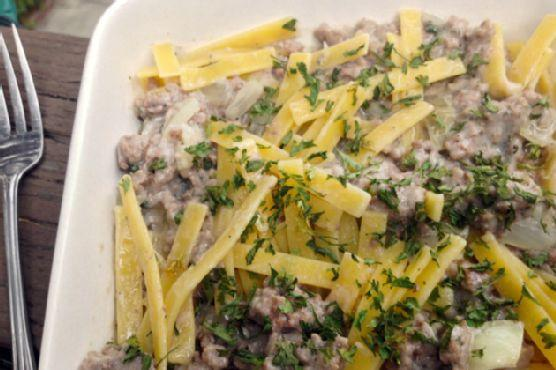
\includegraphics[width=\linewidth]{images/evaluation-images/beef_stroganoff/beef-stroganoff122.jpg}
\end{minipage}
\hfill
\begin{minipage}[t]{0.5\textwidth}
	\vspace{0pt}\raggedright
	\begin{tabularx}{\textwidth}{X r}
		\small \textbf{Real class} & \small Beef Stroganoff\\
		\small \textbf{Predicted class} & \small Nachos\\
		\small \textbf{Predicted accuracy} & \small 29.72 \%
    \end{tabularx}\\
    
    \vspace{6pt}
	\begin{tabularx}{\textwidth}{X r}
        \small \textbf{Top-5} & \small \textbf{Accuracy} \\
        \hline
		\small 1) Nachos & \small 29.72 \%\\\small 2) Salad & \small 23.57 \%\\\small 3) Pizza & \small 14.29 \%\\\small 4) Coleslaw & \small 10.63 \%\\\small 5) Caesar Salad & \small 3.75 \%
    \end{tabularx}
\end{minipage}
    
\subsection{Brownies}
    
\subsubsection{brownies/brownies224.jpg}

\begin{minipage}[t]{0.4\textwidth}
	\vspace{0pt}
	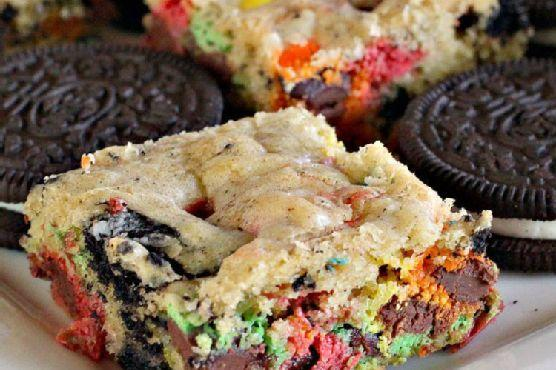
\includegraphics[width=\linewidth]{images/evaluation-images/brownies/brownies224.jpg}
\end{minipage}
\hfill
\begin{minipage}[t]{0.5\textwidth}
	\vspace{0pt}\raggedright
	\begin{tabularx}{\textwidth}{X r}
		\small \textbf{Real class} & \small Brownies\\
		\small \textbf{Predicted class} & \small Cinnamon Roll\\
		\small \textbf{Predicted accuracy} & \small 62.64 \%
    \end{tabularx}\\
    
    \vspace{6pt}
	\begin{tabularx}{\textwidth}{X r}
        \small \textbf{Top-5} & \small \textbf{Accuracy} \\
        \hline
		\small 1) Cinnamon Roll & \small 62.64 \%\\\small 2) Muffin & \small 11.39 \%\\\small 3) Meatloaf & \small 6.08 \%\\\small 4) Bundt Cake & \small 5.64 \%\\\small 5) Frittata & \small 3.13 \%
    \end{tabularx}
\end{minipage}
    
\subsection{Burger}
    
\subsubsection{burger/burger188.jpeg}

\begin{minipage}[t]{0.4\textwidth}
	\vspace{0pt}
	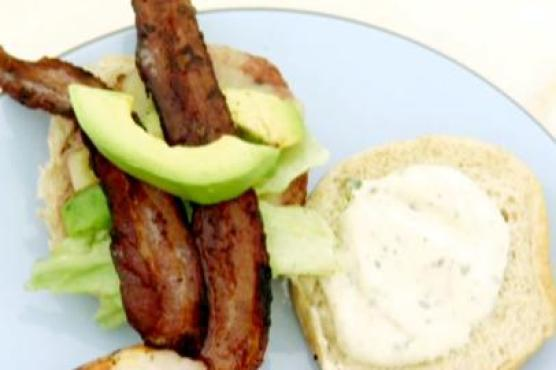
\includegraphics[width=\linewidth]{images/evaluation-images/burger/burger188.jpeg}
\end{minipage}
\hfill
\begin{minipage}[t]{0.5\textwidth}
	\vspace{0pt}\raggedright
	\begin{tabularx}{\textwidth}{X r}
		\small \textbf{Real class} & \small Burger\\
		\small \textbf{Predicted class} & \small Kebabs\\
		\small \textbf{Predicted accuracy} & \small 47.61 \%
    \end{tabularx}\\
    
    \vspace{6pt}
	\begin{tabularx}{\textwidth}{X r}
        \small \textbf{Top-5} & \small \textbf{Accuracy} \\
        \hline
		\small 1) Kebabs & \small 47.61 \%\\\small 2) Ice Cream & \small 13.01 \%\\\small 3) Chicken Wings & \small 10.95 \%\\\small 4) Meatballs & \small 9.61 \%\\\small 5) French Fries & \small 2.45 \%
    \end{tabularx}
\end{minipage}
    
\subsubsection{burger/burger30.jpg}

\begin{minipage}[t]{0.4\textwidth}
	\vspace{0pt}
	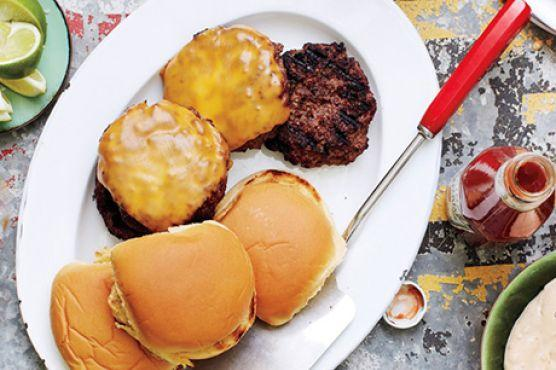
\includegraphics[width=\linewidth]{images/evaluation-images/burger/burger30.jpg}
\end{minipage}
\hfill
\begin{minipage}[t]{0.5\textwidth}
	\vspace{0pt}\raggedright
	\begin{tabularx}{\textwidth}{X r}
		\small \textbf{Real class} & \small Burger\\
		\small \textbf{Predicted class} & \small Stuffed Pepper\\
		\small \textbf{Predicted accuracy} & \small 34.01 \%
    \end{tabularx}\\
    
    \vspace{6pt}
	\begin{tabularx}{\textwidth}{X r}
        \small \textbf{Top-5} & \small \textbf{Accuracy} \\
        \hline
		\small 1) Stuffed Pepper & \small 34.01 \%\\\small 2) Corn Dog & \small 12.83 \%\\\small 3) Muffin & \small 12.60 \%\\\small 4) Kebabs & \small 12.48 \%\\\small 5) Meatballs & \small 10.81 \%
    \end{tabularx}
\end{minipage}
    
\subsection{Burrito}
    
\subsubsection{burrito/burrito99.jpg}

\begin{minipage}[t]{0.4\textwidth}
	\vspace{0pt}
	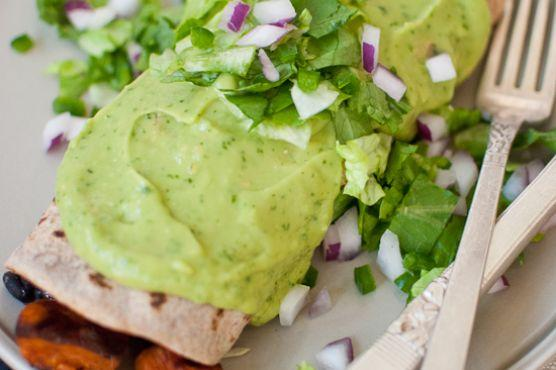
\includegraphics[width=\linewidth]{images/evaluation-images/burrito/burrito99.jpg}
\end{minipage}
\hfill
\begin{minipage}[t]{0.5\textwidth}
	\vspace{0pt}\raggedright
	\begin{tabularx}{\textwidth}{X r}
		\small \textbf{Real class} & \small Burrito\\
		\small \textbf{Predicted class} & \small Guacamole\\
		\small \textbf{Predicted accuracy} & \small 74.97 \%
    \end{tabularx}\\
    
    \vspace{6pt}
	\begin{tabularx}{\textwidth}{X r}
        \small \textbf{Top-5} & \small \textbf{Accuracy} \\
        \hline
		\small 1) Guacamole & \small 74.97 \%\\\small 2) Nachos & \small 5.24 \%\\\small 3) Omelet & \small 4.87 \%\\\small 4) Salad & \small 3.54 \%\\\small 5) Quesadilla & \small 2.44 \%
    \end{tabularx}
\end{minipage}
    
\subsection{Caesar Salad}
    
\subsubsection{caesar\textunderscore salad/caesar-salad110.jpg}

\begin{minipage}[t]{0.4\textwidth}
	\vspace{0pt}
	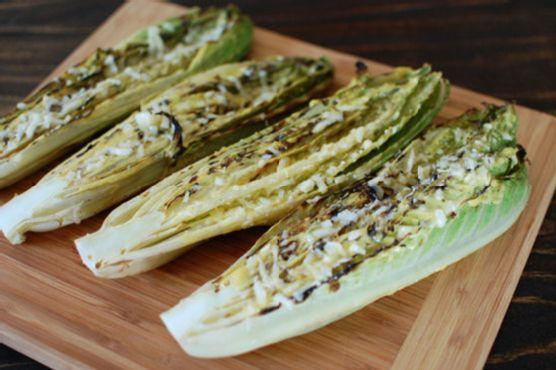
\includegraphics[width=\linewidth]{images/evaluation-images/caesar_salad/caesar-salad110.jpg}
\end{minipage}
\hfill
\begin{minipage}[t]{0.5\textwidth}
	\vspace{0pt}\raggedright
	\begin{tabularx}{\textwidth}{X r}
		\small \textbf{Real class} & \small Caesar Salad\\
		\small \textbf{Predicted class} & \small Quesadilla\\
		\small \textbf{Predicted accuracy} & \small 84.89 \%
    \end{tabularx}\\
    
    \vspace{6pt}
	\begin{tabularx}{\textwidth}{X r}
        \small \textbf{Top-5} & \small \textbf{Accuracy} \\
        \hline
		\small 1) Quesadilla & \small 84.89 \%\\\small 2) Frittata & \small 10.50 \%\\\small 3) Granola Bar & \small 1.05 \%\\\small 4) Baked Salmon & \small 1.04 \%\\\small 5) Grilled Cheese Sandwich & \small 0.65 \%
    \end{tabularx}
\end{minipage}
    
\subsubsection{caesar\textunderscore salad/caesar-salad193.jpg}

\begin{minipage}[t]{0.4\textwidth}
	\vspace{0pt}
	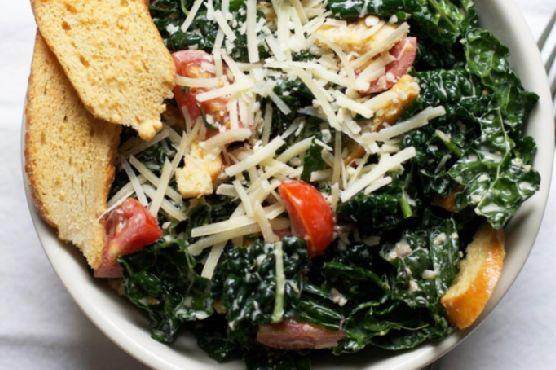
\includegraphics[width=\linewidth]{images/evaluation-images/caesar_salad/caesar-salad193.jpg}
\end{minipage}
\hfill
\begin{minipage}[t]{0.5\textwidth}
	\vspace{0pt}\raggedright
	\begin{tabularx}{\textwidth}{X r}
		\small \textbf{Real class} & \small Caesar Salad\\
		\small \textbf{Predicted class} & \small Salad\\
		\small \textbf{Predicted accuracy} & \small 95.82 \%
    \end{tabularx}\\
    
    \vspace{6pt}
	\begin{tabularx}{\textwidth}{X r}
        \small \textbf{Top-5} & \small \textbf{Accuracy} \\
        \hline
		\small 1) Salad & \small 95.82 \%\\\small 2) Omelet & \small 3.07 \%\\\small 3) Coleslaw & \small 0.25 \%\\\small 4) Creamed Spinach & \small 0.24 \%\\\small 5) Cobb Salad & \small 0.20 \%
    \end{tabularx}
\end{minipage}
    
\subsection{Calzone}
    
\subsubsection{calzone/calzone172.jpg}

\begin{minipage}[t]{0.4\textwidth}
	\vspace{0pt}
	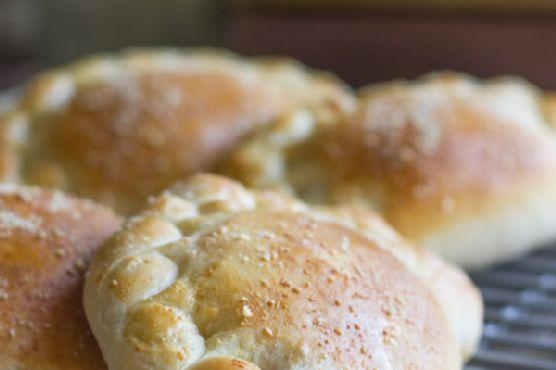
\includegraphics[width=\linewidth]{images/evaluation-images/calzone/calzone172.jpg}
\end{minipage}
\hfill
\begin{minipage}[t]{0.5\textwidth}
	\vspace{0pt}\raggedright
	\begin{tabularx}{\textwidth}{X r}
		\small \textbf{Real class} & \small Calzone\\
		\small \textbf{Predicted class} & \small Buttermilk Biscuits\\
		\small \textbf{Predicted accuracy} & \small 44.04 \%
    \end{tabularx}\\
    
    \vspace{6pt}
	\begin{tabularx}{\textwidth}{X r}
        \small \textbf{Top-5} & \small \textbf{Accuracy} \\
        \hline
		\small 1) Buttermilk Biscuits & \small 44.04 \%\\\small 2) Muffin & \small 40.37 \%\\\small 3) Empanada & \small 8.33 \%\\\small 4) Donut & \small 3.51 \%\\\small 5) Pancakes & \small 2.59 \%
    \end{tabularx}
\end{minipage}
    
\subsubsection{calzone/calzone73.jpg}

\begin{minipage}[t]{0.4\textwidth}
	\vspace{0pt}
	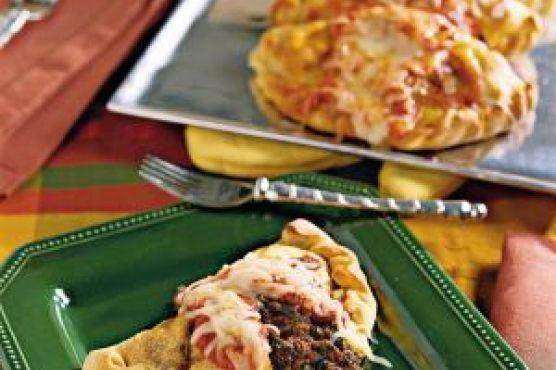
\includegraphics[width=\linewidth]{images/evaluation-images/calzone/calzone73.jpg}
\end{minipage}
\hfill
\begin{minipage}[t]{0.5\textwidth}
	\vspace{0pt}\raggedright
	\begin{tabularx}{\textwidth}{X r}
		\small \textbf{Real class} & \small Calzone\\
		\small \textbf{Predicted class} & \small Muffin\\
		\small \textbf{Predicted accuracy} & \small 35.20 \%
    \end{tabularx}\\
    
    \vspace{6pt}
	\begin{tabularx}{\textwidth}{X r}
        \small \textbf{Top-5} & \small \textbf{Accuracy} \\
        \hline
		\small 1) Muffin & \small 35.20 \%\\\small 2) Omelet & \small 27.60 \%\\\small 3) Pizza & \small 6.56 \%\\\small 4) Frittata & \small 5.95 \%\\\small 5) Nachos & \small 4.22 \%
    \end{tabularx}
\end{minipage}
    
\subsection{Cheesecake}
    
\subsubsection{cheesecake/cheesecake147.jpg}

\begin{minipage}[t]{0.4\textwidth}
	\vspace{0pt}
	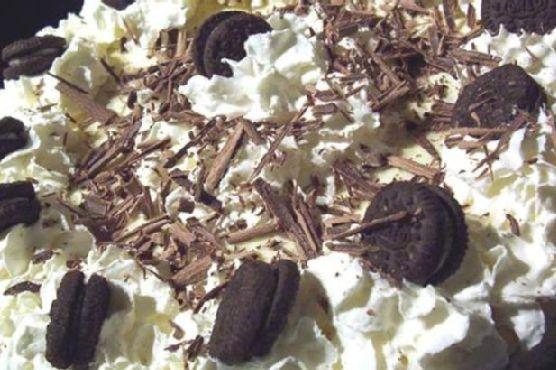
\includegraphics[width=\linewidth]{images/evaluation-images/cheesecake/cheesecake147.jpg}
\end{minipage}
\hfill
\begin{minipage}[t]{0.5\textwidth}
	\vspace{0pt}\raggedright
	\begin{tabularx}{\textwidth}{X r}
		\small \textbf{Real class} & \small Cheesecake\\
		\small \textbf{Predicted class} & \small Creamed Spinach\\
		\small \textbf{Predicted accuracy} & \small 34.59 \%
    \end{tabularx}\\
    
    \vspace{6pt}
	\begin{tabularx}{\textwidth}{X r}
        \small \textbf{Top-5} & \small \textbf{Accuracy} \\
        \hline
		\small 1) Creamed Spinach & \small 34.59 \%\\\small 2) Popcorn & \small 18.25 \%\\\small 3) Coleslaw & \small 13.17 \%\\\small 4) Bundt Cake & \small 8.06 \%\\\small 5) Meatballs & \small 6.06 \%
    \end{tabularx}
\end{minipage}
    
\subsubsection{cheesecake/cheesecake409.jpg}

\begin{minipage}[t]{0.4\textwidth}
	\vspace{0pt}
	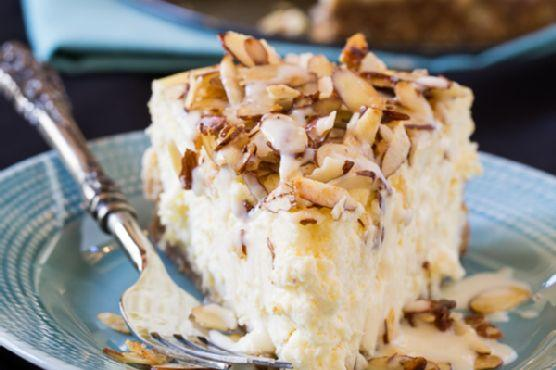
\includegraphics[width=\linewidth]{images/evaluation-images/cheesecake/cheesecake409.jpg}
\end{minipage}
\hfill
\begin{minipage}[t]{0.5\textwidth}
	\vspace{0pt}\raggedright
	\begin{tabularx}{\textwidth}{X r}
		\small \textbf{Real class} & \small Cheesecake\\
		\small \textbf{Predicted class} & \small Cinnamon Roll\\
		\small \textbf{Predicted accuracy} & \small 95.37 \%
    \end{tabularx}\\
    
    \vspace{6pt}
	\begin{tabularx}{\textwidth}{X r}
        \small \textbf{Top-5} & \small \textbf{Accuracy} \\
        \hline
		\small 1) Cinnamon Roll & \small 95.37 \%\\\small 2) Ice Cream & \small 2.00 \%\\\small 3) Mashed Potatoes & \small 1.95 \%\\\small 4) Burrito & \small 0.28 \%\\\small 5) Coleslaw & \small 0.08 \%
    \end{tabularx}
\end{minipage}
    
\subsection{Cinnamon Roll}
    
\subsubsection{cinnamon\textunderscore roll/cinnamon-roll256.jpg}

\begin{minipage}[t]{0.4\textwidth}
	\vspace{0pt}
	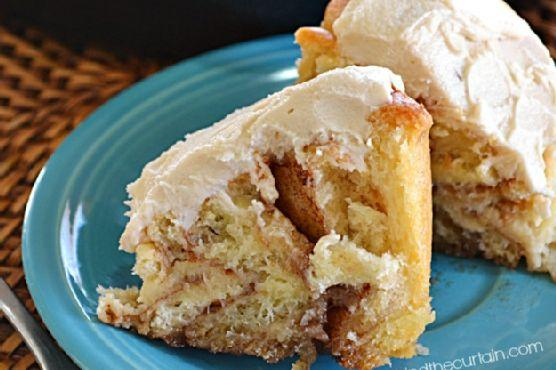
\includegraphics[width=\linewidth]{images/evaluation-images/cinnamon_roll/cinnamon-roll256.jpg}
\end{minipage}
\hfill
\begin{minipage}[t]{0.5\textwidth}
	\vspace{0pt}\raggedright
	\begin{tabularx}{\textwidth}{X r}
		\small \textbf{Real class} & \small Cinnamon Roll\\
		\small \textbf{Predicted class} & \small Empanada\\
		\small \textbf{Predicted accuracy} & \small 95.06 \%
    \end{tabularx}\\
    
    \vspace{6pt}
	\begin{tabularx}{\textwidth}{X r}
        \small \textbf{Top-5} & \small \textbf{Accuracy} \\
        \hline
		\small 1) Empanada & \small 95.06 \%\\\small 2) Calzone & \small 3.84 \%\\\small 3) Ice Cream & \small 0.69 \%\\\small 4) Buttermilk Biscuits & \small 0.13 \%\\\small 5) Muffin & \small 0.08 \%
    \end{tabularx}
\end{minipage}
    
\subsubsection{cinnamon\textunderscore roll/cinnamon-roll384.jpg}

\begin{minipage}[t]{0.4\textwidth}
	\vspace{0pt}
	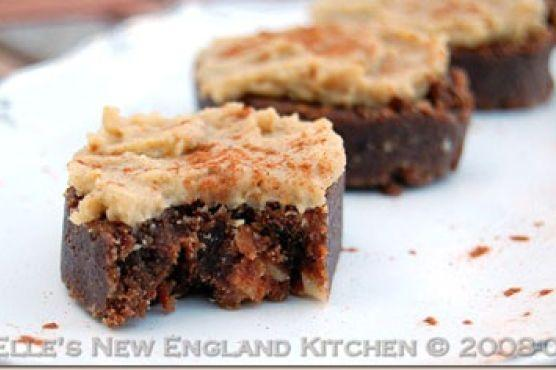
\includegraphics[width=\linewidth]{images/evaluation-images/cinnamon_roll/cinnamon-roll384.jpg}
\end{minipage}
\hfill
\begin{minipage}[t]{0.5\textwidth}
	\vspace{0pt}\raggedright
	\begin{tabularx}{\textwidth}{X r}
		\small \textbf{Real class} & \small Cinnamon Roll\\
		\small \textbf{Predicted class} & \small Brownies\\
		\small \textbf{Predicted accuracy} & \small 98.75 \%
    \end{tabularx}\\
    
    \vspace{6pt}
	\begin{tabularx}{\textwidth}{X r}
        \small \textbf{Top-5} & \small \textbf{Accuracy} \\
        \hline
		\small 1) Brownies & \small 98.75 \%\\\small 2) Lasagne & \small 1.06 \%\\\small 3) Grilled Cheese Sandwich & \small 0.05 \%\\\small 4) Muffin & \small 0.04 \%\\\small 5) Granola Bar & \small 0.02 \%
    \end{tabularx}
\end{minipage}
    
\subsection{Corn Dog}
    
\subsubsection{corn\textunderscore dog/corn-dog25.jpg}

\begin{minipage}[t]{0.4\textwidth}
	\vspace{0pt}
	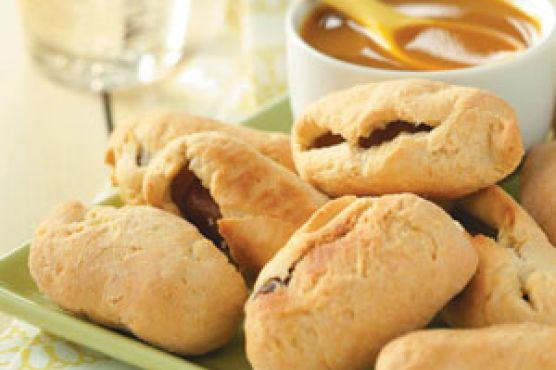
\includegraphics[width=\linewidth]{images/evaluation-images/corn_dog/corn-dog25.jpg}
\end{minipage}
\hfill
\begin{minipage}[t]{0.5\textwidth}
	\vspace{0pt}\raggedright
	\begin{tabularx}{\textwidth}{X r}
		\small \textbf{Real class} & \small Corn Dog\\
		\small \textbf{Predicted class} & \small Empanada\\
		\small \textbf{Predicted accuracy} & \small 99.83 \%
    \end{tabularx}\\
    
    \vspace{6pt}
	\begin{tabularx}{\textwidth}{X r}
        \small \textbf{Top-5} & \small \textbf{Accuracy} \\
        \hline
		\small 1) Empanada & \small 99.83 \%\\\small 2) Buttermilk Biscuits & \small 0.08 \%\\\small 3) Muffin & \small 0.05 \%\\\small 4) Calzone & \small 0.03 \%\\\small 5) Chicken Wings & \small 0.00 \%
    \end{tabularx}
\end{minipage}
    
\subsection{Donut}
    
\subsubsection{donut/donut408.jpg}

\begin{minipage}[t]{0.4\textwidth}
	\vspace{0pt}
	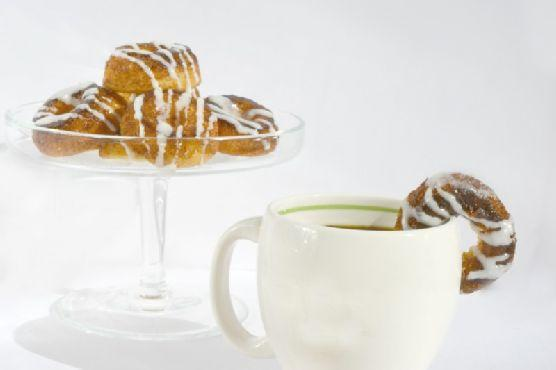
\includegraphics[width=\linewidth]{images/evaluation-images/donut/donut408.jpg}
\end{minipage}
\hfill
\begin{minipage}[t]{0.5\textwidth}
	\vspace{0pt}\raggedright
	\begin{tabularx}{\textwidth}{X r}
		\small \textbf{Real class} & \small Donut\\
		\small \textbf{Predicted class} & \small Margarita\\
		\small \textbf{Predicted accuracy} & \small 51.65 \%
    \end{tabularx}\\
    
    \vspace{6pt}
	\begin{tabularx}{\textwidth}{X r}
        \small \textbf{Top-5} & \small \textbf{Accuracy} \\
        \hline
		\small 1) Margarita & \small 51.65 \%\\\small 2) Martini & \small 7.32 \%\\\small 3) Kebabs & \small 5.00 \%\\\small 4) Bundt Cake & \small 2.89 \%\\\small 5) Cinnamon Roll & \small 2.87 \%
    \end{tabularx}
\end{minipage}
    
\subsection{Empanada}
    
\subsubsection{empanada/empanada118.jpg}

\begin{minipage}[t]{0.4\textwidth}
	\vspace{0pt}
	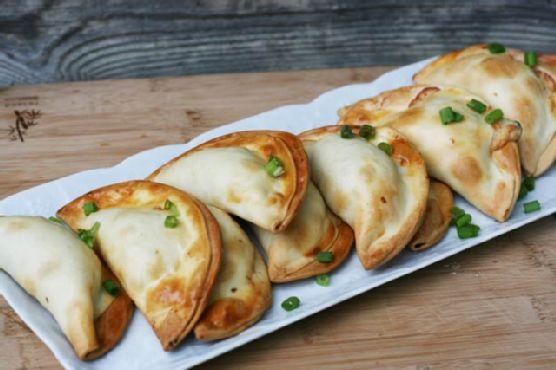
\includegraphics[width=\linewidth]{images/evaluation-images/empanada/empanada118.jpg}
\end{minipage}
\hfill
\begin{minipage}[t]{0.5\textwidth}
	\vspace{0pt}\raggedright
	\begin{tabularx}{\textwidth}{X r}
		\small \textbf{Real class} & \small Empanada\\
		\small \textbf{Predicted class} & \small Kebabs\\
		\small \textbf{Predicted accuracy} & \small 65.94 \%
    \end{tabularx}\\
    
    \vspace{6pt}
	\begin{tabularx}{\textwidth}{X r}
        \small \textbf{Top-5} & \small \textbf{Accuracy} \\
        \hline
		\small 1) Kebabs & \small 65.94 \%\\\small 2) Quesadilla & \small 22.44 \%\\\small 3) Burrito & \small 10.49 \%\\\small 4) Calzone & \small 0.51 \%\\\small 5) Corn Dog & \small 0.16 \%
    \end{tabularx}
\end{minipage}
    
\subsubsection{empanada/empanada154.jpg}

\begin{minipage}[t]{0.4\textwidth}
	\vspace{0pt}
	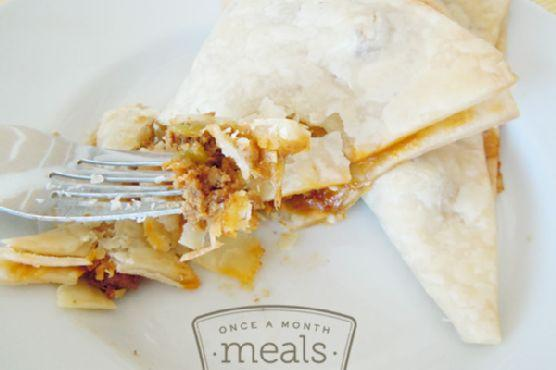
\includegraphics[width=\linewidth]{images/evaluation-images/empanada/empanada154.jpg}
\end{minipage}
\hfill
\begin{minipage}[t]{0.5\textwidth}
	\vspace{0pt}\raggedright
	\begin{tabularx}{\textwidth}{X r}
		\small \textbf{Real class} & \small Empanada\\
		\small \textbf{Predicted class} & \small Quesadilla\\
		\small \textbf{Predicted accuracy} & \small 99.98 \%
    \end{tabularx}\\
    
    \vspace{6pt}
	\begin{tabularx}{\textwidth}{X r}
        \small \textbf{Top-5} & \small \textbf{Accuracy} \\
        \hline
		\small 1) Quesadilla & \small 99.98 \%\\\small 2) Burrito & \small 0.00 \%\\\small 3) French Fries & \small 0.00 \%\\\small 4) Coleslaw & \small 0.00 \%\\\small 5) Kebabs & \small 0.00 \%
    \end{tabularx}
\end{minipage}
    
\subsubsection{empanada/empanada34.jpg}

\begin{minipage}[t]{0.4\textwidth}
	\vspace{0pt}
	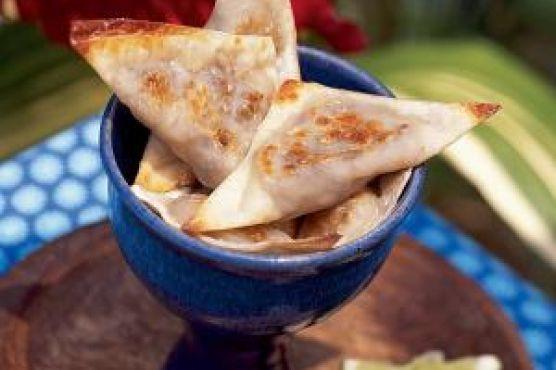
\includegraphics[width=\linewidth]{images/evaluation-images/empanada/empanada34.jpg}
\end{minipage}
\hfill
\begin{minipage}[t]{0.5\textwidth}
	\vspace{0pt}\raggedright
	\begin{tabularx}{\textwidth}{X r}
		\small \textbf{Real class} & \small Empanada\\
		\small \textbf{Predicted class} & \small Quesadilla\\
		\small \textbf{Predicted accuracy} & \small 97.91 \%
    \end{tabularx}\\
    
    \vspace{6pt}
	\begin{tabularx}{\textwidth}{X r}
        \small \textbf{Top-5} & \small \textbf{Accuracy} \\
        \hline
		\small 1) Quesadilla & \small 97.91 \%\\\small 2) Burrito & \small 1.28 \%\\\small 3) Martini & \small 0.12 \%\\\small 4) Ice Cream & \small 0.12 \%\\\small 5) Margarita & \small 0.11 \%
    \end{tabularx}
\end{minipage}
    
\subsection{French Fries}
    
\subsubsection{french\textunderscore fries/french-fries19.jpg}

\begin{minipage}[t]{0.4\textwidth}
	\vspace{0pt}
	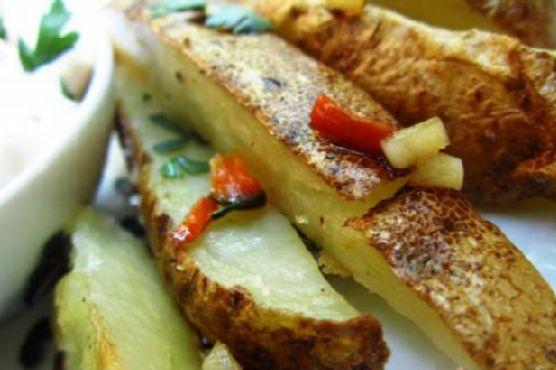
\includegraphics[width=\linewidth]{images/evaluation-images/french_fries/french-fries19.jpg}
\end{minipage}
\hfill
\begin{minipage}[t]{0.5\textwidth}
	\vspace{0pt}\raggedright
	\begin{tabularx}{\textwidth}{X r}
		\small \textbf{Real class} & \small French Fries\\
		\small \textbf{Predicted class} & \small Grilled Cheese Sandwich\\
		\small \textbf{Predicted accuracy} & \small 27.73 \%
    \end{tabularx}\\
    
    \vspace{6pt}
	\begin{tabularx}{\textwidth}{X r}
        \small \textbf{Top-5} & \small \textbf{Accuracy} \\
        \hline
		\small 1) Grilled Cheese Sandwich & \small 27.73 \%\\\small 2) Kebabs & \small 14.09 \%\\\small 3) Quesadilla & \small 13.09 \%\\\small 4) Caesar Salad & \small 12.24 \%\\\small 5) Meatloaf & \small 9.36 \%
    \end{tabularx}
\end{minipage}
    
\subsection{Frittata}
    
\subsubsection{frittata/frittata101.jpg}

\begin{minipage}[t]{0.4\textwidth}
	\vspace{0pt}
	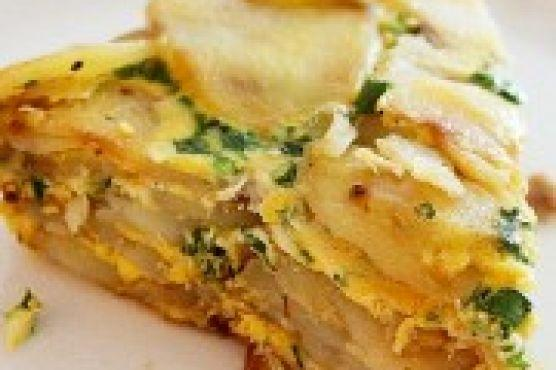
\includegraphics[width=\linewidth]{images/evaluation-images/frittata/frittata101.jpg}
\end{minipage}
\hfill
\begin{minipage}[t]{0.5\textwidth}
	\vspace{0pt}\raggedright
	\begin{tabularx}{\textwidth}{X r}
		\small \textbf{Real class} & \small Frittata\\
		\small \textbf{Predicted class} & \small Chicken Piccata\\
		\small \textbf{Predicted accuracy} & \small 76.85 \%
    \end{tabularx}\\
    
    \vspace{6pt}
	\begin{tabularx}{\textwidth}{X r}
        \small \textbf{Top-5} & \small \textbf{Accuracy} \\
        \hline
		\small 1) Chicken Piccata & \small 76.85 \%\\\small 2) Chicken Wings & \small 3.62 \%\\\small 3) Lasagne & \small 3.15 \%\\\small 4) Omelet & \small 3.11 \%\\\small 5) Kebabs & \small 2.49 \%
    \end{tabularx}
\end{minipage}
    
\subsubsection{frittata/frittata275.jpg}

\begin{minipage}[t]{0.4\textwidth}
	\vspace{0pt}
	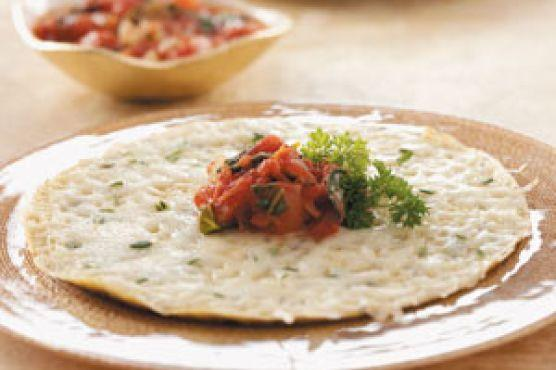
\includegraphics[width=\linewidth]{images/evaluation-images/frittata/frittata275.jpg}
\end{minipage}
\hfill
\begin{minipage}[t]{0.5\textwidth}
	\vspace{0pt}\raggedright
	\begin{tabularx}{\textwidth}{X r}
		\small \textbf{Real class} & \small Frittata\\
		\small \textbf{Predicted class} & \small Omelet\\
		\small \textbf{Predicted accuracy} & \small 37.86 \%
    \end{tabularx}\\
    
    \vspace{6pt}
	\begin{tabularx}{\textwidth}{X r}
        \small \textbf{Top-5} & \small \textbf{Accuracy} \\
        \hline
		\small 1) Omelet & \small 37.86 \%\\\small 2) Quesadilla & \small 30.25 \%\\\small 3) Pancakes & \small 22.37 \%\\\small 4) Pizza & \small 7.01 \%\\\small 5) Chicken Piccata & \small 0.79 \%
    \end{tabularx}
\end{minipage}
    
\subsubsection{frittata/frittata364.jpg}

\begin{minipage}[t]{0.4\textwidth}
	\vspace{0pt}
	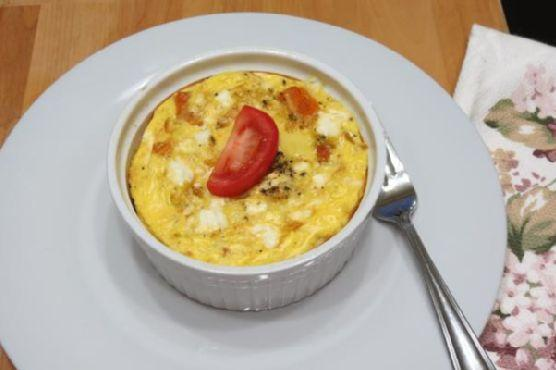
\includegraphics[width=\linewidth]{images/evaluation-images/frittata/frittata364.jpg}
\end{minipage}
\hfill
\begin{minipage}[t]{0.5\textwidth}
	\vspace{0pt}\raggedright
	\begin{tabularx}{\textwidth}{X r}
		\small \textbf{Real class} & \small Frittata\\
		\small \textbf{Predicted class} & \small Macaroni And Cheese\\
		\small \textbf{Predicted accuracy} & \small 97.06 \%
    \end{tabularx}\\
    
    \vspace{6pt}
	\begin{tabularx}{\textwidth}{X r}
        \small \textbf{Top-5} & \small \textbf{Accuracy} \\
        \hline
		\small 1) Macaroni And Cheese & \small 97.06 \%\\\small 2) Omelet & \small 1.81 \%\\\small 3) Lasagne & \small 0.41 \%\\\small 4) Soup & \small 0.23 \%\\\small 5) Baked Beans & \small 0.16 \%
    \end{tabularx}
\end{minipage}
    
\subsubsection{frittata/frittata435.jpg}

\begin{minipage}[t]{0.4\textwidth}
	\vspace{0pt}
	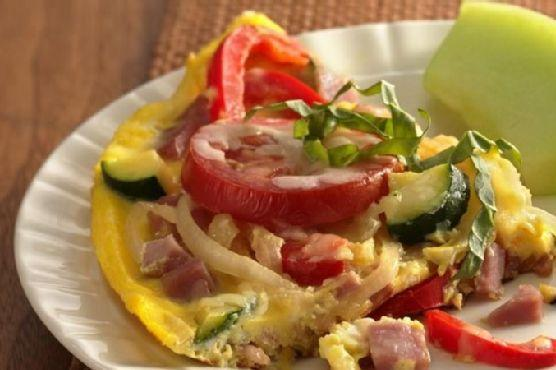
\includegraphics[width=\linewidth]{images/evaluation-images/frittata/frittata435.jpg}
\end{minipage}
\hfill
\begin{minipage}[t]{0.5\textwidth}
	\vspace{0pt}\raggedright
	\begin{tabularx}{\textwidth}{X r}
		\small \textbf{Real class} & \small Frittata\\
		\small \textbf{Predicted class} & \small Stuffed Pepper\\
		\small \textbf{Predicted accuracy} & \small 49.74 \%
    \end{tabularx}\\
    
    \vspace{6pt}
	\begin{tabularx}{\textwidth}{X r}
        \small \textbf{Top-5} & \small \textbf{Accuracy} \\
        \hline
		\small 1) Stuffed Pepper & \small 49.74 \%\\\small 2) Cobb Salad & \small 9.06 \%\\\small 3) Coleslaw & \small 8.23 \%\\\small 4) Burger & \small 7.09 \%\\\small 5) Salad & \small 5.76 \%
    \end{tabularx}
\end{minipage}
    
\subsubsection{frittata/frittata476.jpg}

\begin{minipage}[t]{0.4\textwidth}
	\vspace{0pt}
	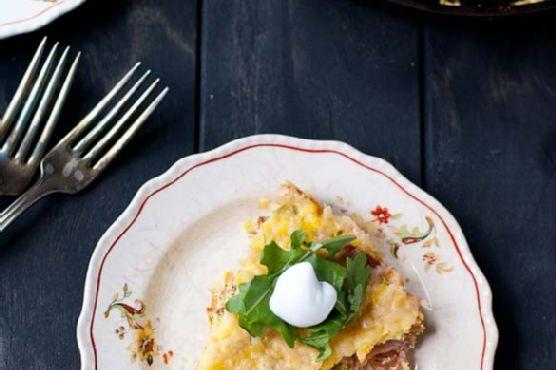
\includegraphics[width=\linewidth]{images/evaluation-images/frittata/frittata476.jpg}
\end{minipage}
\hfill
\begin{minipage}[t]{0.5\textwidth}
	\vspace{0pt}\raggedright
	\begin{tabularx}{\textwidth}{X r}
		\small \textbf{Real class} & \small Frittata\\
		\small \textbf{Predicted class} & \small Soup\\
		\small \textbf{Predicted accuracy} & \small 92.12 \%
    \end{tabularx}\\
    
    \vspace{6pt}
	\begin{tabularx}{\textwidth}{X r}
        \small \textbf{Top-5} & \small \textbf{Accuracy} \\
        \hline
		\small 1) Soup & \small 92.12 \%\\\small 2) Key Lime Pie & \small 1.38 \%\\\small 3) Nachos & \small 1.02 \%\\\small 4) Omelet & \small 0.79 \%\\\small 5) Guacamole & \small 0.66 \%
    \end{tabularx}
\end{minipage}
    
\subsubsection{frittata/frittata73.jpeg}

\begin{minipage}[t]{0.4\textwidth}
	\vspace{0pt}
	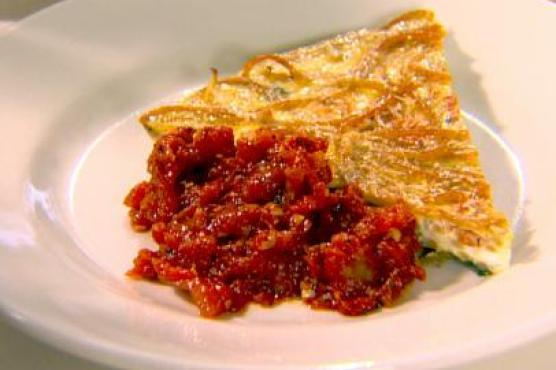
\includegraphics[width=\linewidth]{images/evaluation-images/frittata/frittata73.jpeg}
\end{minipage}
\hfill
\begin{minipage}[t]{0.5\textwidth}
	\vspace{0pt}\raggedright
	\begin{tabularx}{\textwidth}{X r}
		\small \textbf{Real class} & \small Frittata\\
		\small \textbf{Predicted class} & \small Waffles\\
		\small \textbf{Predicted accuracy} & \small 61.02 \%
    \end{tabularx}\\
    
    \vspace{6pt}
	\begin{tabularx}{\textwidth}{X r}
        \small \textbf{Top-5} & \small \textbf{Accuracy} \\
        \hline
		\small 1) Waffles & \small 61.02 \%\\\small 2) Omelet & \small 18.26 \%\\\small 3) Baked Beans & \small 13.17 \%\\\small 4) Lasagne & \small 1.78 \%\\\small 5) Cheesecake & \small 1.28 \%
    \end{tabularx}
\end{minipage}
    
\subsection{Grilled Cheese Sandwich}
    
\subsubsection{grilled\textunderscore cheese\textunderscore sandwich/grilled-cheese-sandwich448.jpg}

\begin{minipage}[t]{0.4\textwidth}
	\vspace{0pt}
	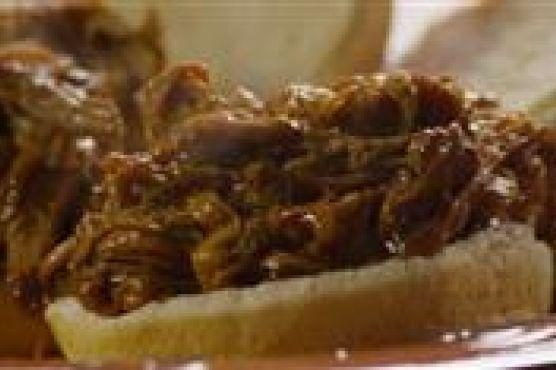
\includegraphics[width=\linewidth]{images/evaluation-images/grilled_cheese_sandwich/grilled-cheese-sandwich448.jpg}
\end{minipage}
\hfill
\begin{minipage}[t]{0.5\textwidth}
	\vspace{0pt}\raggedright
	\begin{tabularx}{\textwidth}{X r}
		\small \textbf{Real class} & \small Grilled Cheese Sandwich\\
		\small \textbf{Predicted class} & \small Waffles\\
		\small \textbf{Predicted accuracy} & \small 66.11 \%
    \end{tabularx}\\
    
    \vspace{6pt}
	\begin{tabularx}{\textwidth}{X r}
        \small \textbf{Top-5} & \small \textbf{Accuracy} \\
        \hline
		\small 1) Waffles & \small 66.11 \%\\\small 2) Pizza & \small 9.49 \%\\\small 3) Lasagne & \small 5.50 \%\\\small 4) Cheesecake & \small 4.67 \%\\\small 5) Brownies & \small 3.70 \%
    \end{tabularx}
\end{minipage}
    
\subsubsection{grilled\textunderscore cheese\textunderscore sandwich/grilled-cheese-sandwich457.jpeg}

\begin{minipage}[t]{0.4\textwidth}
	\vspace{0pt}
	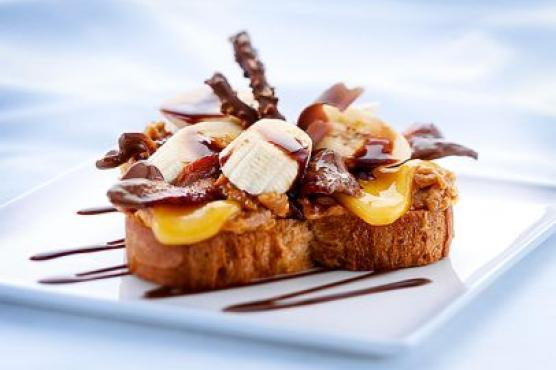
\includegraphics[width=\linewidth]{images/evaluation-images/grilled_cheese_sandwich/grilled-cheese-sandwich457.jpeg}
\end{minipage}
\hfill
\begin{minipage}[t]{0.5\textwidth}
	\vspace{0pt}\raggedright
	\begin{tabularx}{\textwidth}{X r}
		\small \textbf{Real class} & \small Grilled Cheese Sandwich\\
		\small \textbf{Predicted class} & \small Muffin\\
		\small \textbf{Predicted accuracy} & \small 46.27 \%
    \end{tabularx}\\
    
    \vspace{6pt}
	\begin{tabularx}{\textwidth}{X r}
        \small \textbf{Top-5} & \small \textbf{Accuracy} \\
        \hline
		\small 1) Muffin & \small 46.27 \%\\\small 2) Kebabs & \small 13.48 \%\\\small 3) Cinnamon Roll & \small 8.01 \%\\\small 4) Brownies & \small 4.31 \%\\\small 5) Cheesecake & \small 3.70 \%
    \end{tabularx}
\end{minipage}
    
\subsubsection{grilled\textunderscore cheese\textunderscore sandwich/grilled-cheese-sandwich489.jpg}

\begin{minipage}[t]{0.4\textwidth}
	\vspace{0pt}
	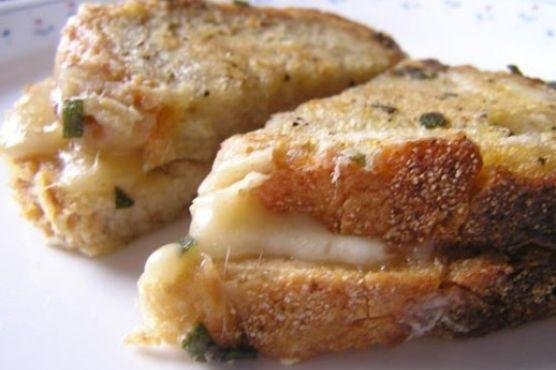
\includegraphics[width=\linewidth]{images/evaluation-images/grilled_cheese_sandwich/grilled-cheese-sandwich489.jpg}
\end{minipage}
\hfill
\begin{minipage}[t]{0.5\textwidth}
	\vspace{0pt}\raggedright
	\begin{tabularx}{\textwidth}{X r}
		\small \textbf{Real class} & \small Grilled Cheese Sandwich\\
		\small \textbf{Predicted class} & \small Frittata\\
		\small \textbf{Predicted accuracy} & \small 92.61 \%
    \end{tabularx}\\
    
    \vspace{6pt}
	\begin{tabularx}{\textwidth}{X r}
        \small \textbf{Top-5} & \small \textbf{Accuracy} \\
        \hline
		\small 1) Frittata & \small 92.61 \%\\\small 2) Baked Salmon & \small 1.73 \%\\\small 3) Meatloaf & \small 1.36 \%\\\small 4) Chicken Piccata & \small 0.83 \%\\\small 5) Omelet & \small 0.67 \%
    \end{tabularx}
\end{minipage}
    
\subsection{Guacamole}
    
\subsubsection{guacamole/guacamole136.jpg}

\begin{minipage}[t]{0.4\textwidth}
	\vspace{0pt}
	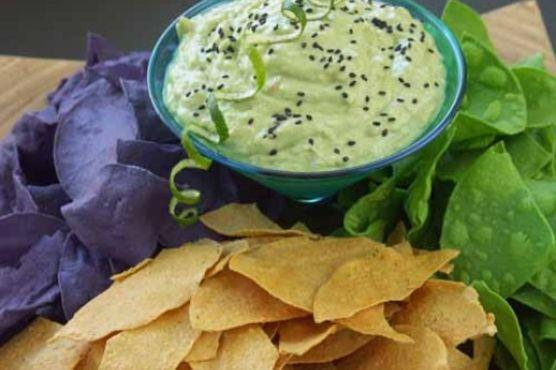
\includegraphics[width=\linewidth]{images/evaluation-images/guacamole/guacamole136.jpg}
\end{minipage}
\hfill
\begin{minipage}[t]{0.5\textwidth}
	\vspace{0pt}\raggedright
	\begin{tabularx}{\textwidth}{X r}
		\small \textbf{Real class} & \small Guacamole\\
		\small \textbf{Predicted class} & \small Margarita\\
		\small \textbf{Predicted accuracy} & \small 22.37 \%
    \end{tabularx}\\
    
    \vspace{6pt}
	\begin{tabularx}{\textwidth}{X r}
        \small \textbf{Top-5} & \small \textbf{Accuracy} \\
        \hline
		\small 1) Margarita & \small 22.37 \%\\\small 2) Mashed Potatoes & \small 19.18 \%\\\small 3) Smoothie & \small 17.14 \%\\\small 4) Pancakes & \small 5.19 \%\\\small 5) Key Lime Pie & \small 4.99 \%
    \end{tabularx}
\end{minipage}
    
\subsection{Ice Cream}
    
\subsubsection{ice\textunderscore cream/ice-cream173.jpg}

\begin{minipage}[t]{0.4\textwidth}
	\vspace{0pt}
	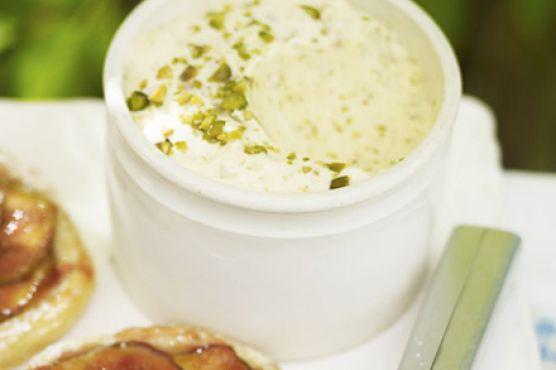
\includegraphics[width=\linewidth]{images/evaluation-images/ice_cream/ice-cream173.jpg}
\end{minipage}
\hfill
\begin{minipage}[t]{0.5\textwidth}
	\vspace{0pt}\raggedright
	\begin{tabularx}{\textwidth}{X r}
		\small \textbf{Real class} & \small Ice Cream\\
		\small \textbf{Predicted class} & \small Key Lime Pie\\
		\small \textbf{Predicted accuracy} & \small 78.80 \%
    \end{tabularx}\\
    
    \vspace{6pt}
	\begin{tabularx}{\textwidth}{X r}
        \small \textbf{Top-5} & \small \textbf{Accuracy} \\
        \hline
		\small 1) Key Lime Pie & \small 78.80 \%\\\small 2) Soup & \small 4.08 \%\\\small 3) Margarita & \small 3.74 \%\\\small 4) Smoothie & \small 1.82 \%\\\small 5) Mashed Potatoes & \small 1.76 \%
    \end{tabularx}
\end{minipage}
    
\subsubsection{ice\textunderscore cream/ice-cream408.jpg}

\begin{minipage}[t]{0.4\textwidth}
	\vspace{0pt}
	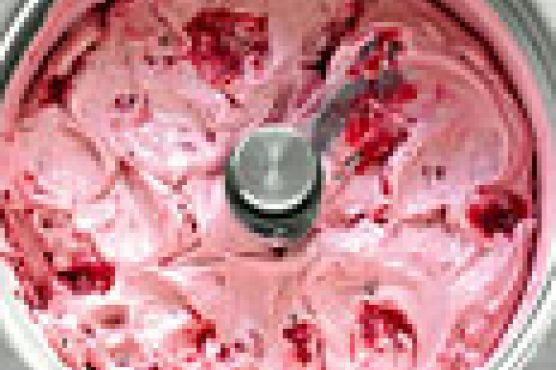
\includegraphics[width=\linewidth]{images/evaluation-images/ice_cream/ice-cream408.jpg}
\end{minipage}
\hfill
\begin{minipage}[t]{0.5\textwidth}
	\vspace{0pt}\raggedright
	\begin{tabularx}{\textwidth}{X r}
		\small \textbf{Real class} & \small Ice Cream\\
		\small \textbf{Predicted class} & \small Bundt Cake\\
		\small \textbf{Predicted accuracy} & \small 97.52 \%
    \end{tabularx}\\
    
    \vspace{6pt}
	\begin{tabularx}{\textwidth}{X r}
        \small \textbf{Top-5} & \small \textbf{Accuracy} \\
        \hline
		\small 1) Bundt Cake & \small 97.52 \%\\\small 2) Cheesecake & \small 1.39 \%\\\small 3) Martini & \small 0.55 \%\\\small 4) Frittata & \small 0.15 \%\\\small 5) Pancakes & \small 0.07 \%
    \end{tabularx}
\end{minipage}
    
\subsection{Kebabs}
    
\subsubsection{kebabs/kebabs136.jpg}

\begin{minipage}[t]{0.4\textwidth}
	\vspace{0pt}
	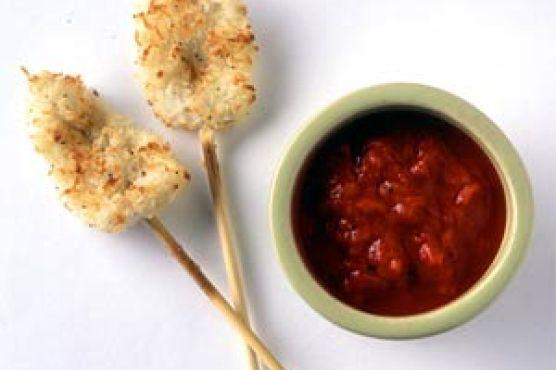
\includegraphics[width=\linewidth]{images/evaluation-images/kebabs/kebabs136.jpg}
\end{minipage}
\hfill
\begin{minipage}[t]{0.5\textwidth}
	\vspace{0pt}\raggedright
	\begin{tabularx}{\textwidth}{X r}
		\small \textbf{Real class} & \small Kebabs\\
		\small \textbf{Predicted class} & \small Soup\\
		\small \textbf{Predicted accuracy} & \small 35.21 \%
    \end{tabularx}\\
    
    \vspace{6pt}
	\begin{tabularx}{\textwidth}{X r}
        \small \textbf{Top-5} & \small \textbf{Accuracy} \\
        \hline
		\small 1) Soup & \small 35.21 \%\\\small 2) Meatballs & \small 34.37 \%\\\small 3) Baked Beans & \small 13.90 \%\\\small 4) Macaroni And Cheese & \small 9.50 \%\\\small 5) Sloppy Joe & \small 0.88 \%
    \end{tabularx}
\end{minipage}
    
\subsubsection{kebabs/kebabs208.png}

\begin{minipage}[t]{0.4\textwidth}
	\vspace{0pt}
	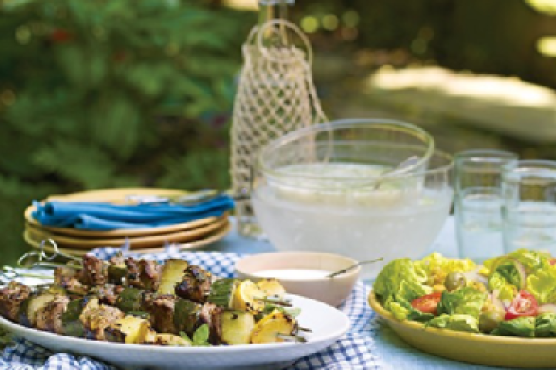
\includegraphics[width=\linewidth]{images/evaluation-images/kebabs/kebabs208.png}
\end{minipage}
\hfill
\begin{minipage}[t]{0.5\textwidth}
	\vspace{0pt}\raggedright
	\begin{tabularx}{\textwidth}{X r}
		\small \textbf{Real class} & \small Kebabs\\
		\small \textbf{Predicted class} & \small Guacamole\\
		\small \textbf{Predicted accuracy} & \small 34.74 \%
    \end{tabularx}\\
    
    \vspace{6pt}
	\begin{tabularx}{\textwidth}{X r}
        \small \textbf{Top-5} & \small \textbf{Accuracy} \\
        \hline
		\small 1) Guacamole & \small 34.74 \%\\\small 2) Salad & \small 19.39 \%\\\small 3) Caesar Salad & \small 18.56 \%\\\small 4) Cobb Salad & \small 11.56 \%\\\small 5) Creamed Spinach & \small 6.77 \%
    \end{tabularx}
\end{minipage}
    
\subsubsection{kebabs/kebabs212.jpg}

\begin{minipage}[t]{0.4\textwidth}
	\vspace{0pt}
	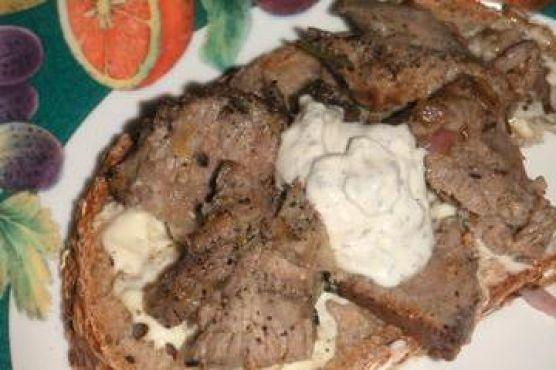
\includegraphics[width=\linewidth]{images/evaluation-images/kebabs/kebabs212.jpg}
\end{minipage}
\hfill
\begin{minipage}[t]{0.5\textwidth}
	\vspace{0pt}\raggedright
	\begin{tabularx}{\textwidth}{X r}
		\small \textbf{Real class} & \small Kebabs\\
		\small \textbf{Predicted class} & \small Meatloaf\\
		\small \textbf{Predicted accuracy} & \small 46.39 \%
    \end{tabularx}\\
    
    \vspace{6pt}
	\begin{tabularx}{\textwidth}{X r}
        \small \textbf{Top-5} & \small \textbf{Accuracy} \\
        \hline
		\small 1) Meatloaf & \small 46.39 \%\\\small 2) Meatballs & \small 34.84 \%\\\small 3) Brownies & \small 5.76 \%\\\small 4) Beef Stroganoff & \small 5.41 \%\\\small 5) Bundt Cake & \small 1.47 \%
    \end{tabularx}
\end{minipage}
    
\subsubsection{kebabs/kebabs218.jpg}

\begin{minipage}[t]{0.4\textwidth}
	\vspace{0pt}
	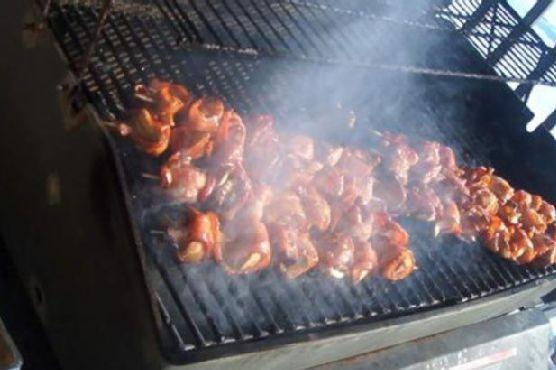
\includegraphics[width=\linewidth]{images/evaluation-images/kebabs/kebabs218.jpg}
\end{minipage}
\hfill
\begin{minipage}[t]{0.5\textwidth}
	\vspace{0pt}\raggedright
	\begin{tabularx}{\textwidth}{X r}
		\small \textbf{Real class} & \small Kebabs\\
		\small \textbf{Predicted class} & \small French Fries\\
		\small \textbf{Predicted accuracy} & \small 18.66 \%
    \end{tabularx}\\
    
    \vspace{6pt}
	\begin{tabularx}{\textwidth}{X r}
        \small \textbf{Top-5} & \small \textbf{Accuracy} \\
        \hline
		\small 1) French Fries & \small 18.66 \%\\\small 2) Baked Salmon & \small 16.28 \%\\\small 3) Grilled Cheese Sandwich & \small 8.70 \%\\\small 4) Cheesecake & \small 7.94 \%\\\small 5) Brownies & \small 6.50 \%
    \end{tabularx}
\end{minipage}
    
\subsubsection{kebabs/kebabs229.jpg}

\begin{minipage}[t]{0.4\textwidth}
	\vspace{0pt}
	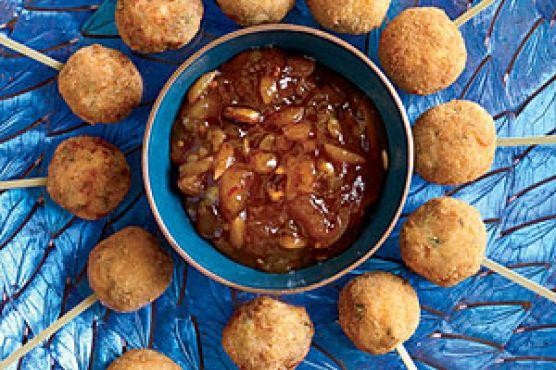
\includegraphics[width=\linewidth]{images/evaluation-images/kebabs/kebabs229.jpg}
\end{minipage}
\hfill
\begin{minipage}[t]{0.5\textwidth}
	\vspace{0pt}\raggedright
	\begin{tabularx}{\textwidth}{X r}
		\small \textbf{Real class} & \small Kebabs\\
		\small \textbf{Predicted class} & \small Muffin\\
		\small \textbf{Predicted accuracy} & \small 81.63 \%
    \end{tabularx}\\
    
    \vspace{6pt}
	\begin{tabularx}{\textwidth}{X r}
        \small \textbf{Top-5} & \small \textbf{Accuracy} \\
        \hline
		\small 1) Muffin & \small 81.63 \%\\\small 2) Meatballs & \small 14.34 \%\\\small 3) Baked Beans & \small 3.51 \%\\\small 4) Pancakes & \small 0.38 \%\\\small 5) Soup & \small 0.03 \%
    \end{tabularx}
\end{minipage}
    
\subsubsection{kebabs/kebabs54.jpg}

\begin{minipage}[t]{0.4\textwidth}
	\vspace{0pt}
	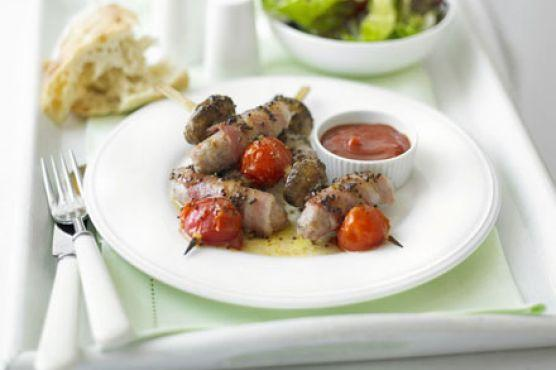
\includegraphics[width=\linewidth]{images/evaluation-images/kebabs/kebabs54.jpg}
\end{minipage}
\hfill
\begin{minipage}[t]{0.5\textwidth}
	\vspace{0pt}\raggedright
	\begin{tabularx}{\textwidth}{X r}
		\small \textbf{Real class} & \small Kebabs\\
		\small \textbf{Predicted class} & \small Soup\\
		\small \textbf{Predicted accuracy} & \small 63.60 \%
    \end{tabularx}\\
    
    \vspace{6pt}
	\begin{tabularx}{\textwidth}{X r}
        \small \textbf{Top-5} & \small \textbf{Accuracy} \\
        \hline
		\small 1) Soup & \small 63.60 \%\\\small 2) Beef Stew & \small 32.90 \%\\\small 3) Salad & \small 1.89 \%\\\small 4) Omelet & \small 0.56 \%\\\small 5) Frittata & \small 0.20 \%
    \end{tabularx}
\end{minipage}
    
\subsubsection{kebabs/kebabs7.jpg}

\begin{minipage}[t]{0.4\textwidth}
	\vspace{0pt}
	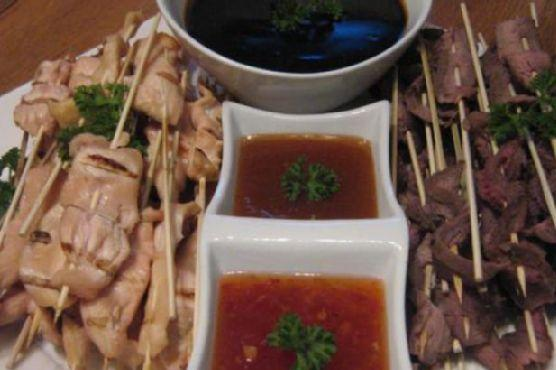
\includegraphics[width=\linewidth]{images/evaluation-images/kebabs/kebabs7.jpg}
\end{minipage}
\hfill
\begin{minipage}[t]{0.5\textwidth}
	\vspace{0pt}\raggedright
	\begin{tabularx}{\textwidth}{X r}
		\small \textbf{Real class} & \small Kebabs\\
		\small \textbf{Predicted class} & \small Soup\\
		\small \textbf{Predicted accuracy} & \small 53.29 \%
    \end{tabularx}\\
    
    \vspace{6pt}
	\begin{tabularx}{\textwidth}{X r}
        \small \textbf{Top-5} & \small \textbf{Accuracy} \\
        \hline
		\small 1) Soup & \small 53.29 \%\\\small 2) Smoothie & \small 25.49 \%\\\small 3) Salad & \small 5.02 \%\\\small 4) Beef Stroganoff & \small 2.82 \%\\\small 5) Coleslaw & \small 2.76 \%
    \end{tabularx}
\end{minipage}
    
\subsection{Lasagne}
    
\subsubsection{lasagne/lasagne181.png}

\begin{minipage}[t]{0.4\textwidth}
	\vspace{0pt}
	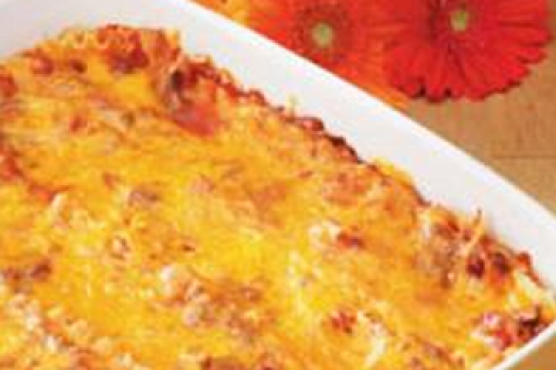
\includegraphics[width=\linewidth]{images/evaluation-images/lasagne/lasagne181.png}
\end{minipage}
\hfill
\begin{minipage}[t]{0.5\textwidth}
	\vspace{0pt}\raggedright
	\begin{tabularx}{\textwidth}{X r}
		\small \textbf{Real class} & \small Lasagne\\
		\small \textbf{Predicted class} & \small Macaroni And Cheese\\
		\small \textbf{Predicted accuracy} & \small 30.00 \%
    \end{tabularx}\\
    
    \vspace{6pt}
	\begin{tabularx}{\textwidth}{X r}
        \small \textbf{Top-5} & \small \textbf{Accuracy} \\
        \hline
		\small 1) Macaroni And Cheese & \small 30.00 \%\\\small 2) Pizza & \small 16.29 \%\\\small 3) Meatballs & \small 16.00 \%\\\small 4) Omelet & \small 10.88 \%\\\small 5) Mashed Potatoes & \small 10.45 \%
    \end{tabularx}
\end{minipage}
    
\subsubsection{lasagne/lasagne449.jpeg}

\begin{minipage}[t]{0.4\textwidth}
	\vspace{0pt}
	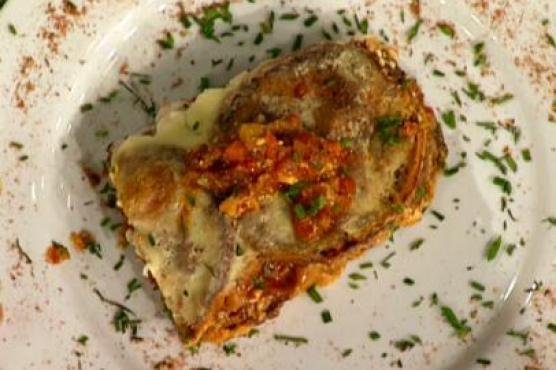
\includegraphics[width=\linewidth]{images/evaluation-images/lasagne/lasagne449.jpeg}
\end{minipage}
\hfill
\begin{minipage}[t]{0.5\textwidth}
	\vspace{0pt}\raggedright
	\begin{tabularx}{\textwidth}{X r}
		\small \textbf{Real class} & \small Lasagne\\
		\small \textbf{Predicted class} & \small Meatloaf\\
		\small \textbf{Predicted accuracy} & \small 49.46 \%
    \end{tabularx}\\
    
    \vspace{6pt}
	\begin{tabularx}{\textwidth}{X r}
        \small \textbf{Top-5} & \small \textbf{Accuracy} \\
        \hline
		\small 1) Meatloaf & \small 49.46 \%\\\small 2) Omelet & \small 30.73 \%\\\small 3) Baked Salmon & \small 7.69 \%\\\small 4) Pizza & \small 6.25 \%\\\small 5) Chicken Piccata & \small 0.96 \%
    \end{tabularx}
\end{minipage}
    
\subsection{Macaroni And Cheese}
    
\subsubsection{macaroni\textunderscore and\textunderscore cheese/macaroni-and-cheese432.jpeg}

\begin{minipage}[t]{0.4\textwidth}
	\vspace{0pt}
	\includegraphics[width=\linewidth]{images/evaluation-images/macaroni_and_cheese/macaroni-and-cheese432.jpeg}
\end{minipage}
\hfill
\begin{minipage}[t]{0.5\textwidth}
	\vspace{0pt}\raggedright
	\begin{tabularx}{\textwidth}{X r}
		\small \textbf{Real class} & \small Macaroni And Cheese\\
		\small \textbf{Predicted class} & \small Grilled Cheese Sandwich\\
		\small \textbf{Predicted accuracy} & \small 99.93 \%
    \end{tabularx}\\
    
    \vspace{6pt}
	\begin{tabularx}{\textwidth}{X r}
        \small \textbf{Top-5} & \small \textbf{Accuracy} \\
        \hline
		\small 1) Grilled Cheese Sandwich & \small 99.93 \%\\\small 2) Burger & \small 0.06 \%\\\small 3) Lasagne & \small 0.00 \%\\\small 4) Sloppy Joe & \small 0.00 \%\\\small 5) Pancakes & \small 0.00 \%
    \end{tabularx}
\end{minipage}
    
\subsubsection{macaroni\textunderscore and\textunderscore cheese/macaroni-and-cheese58.jpg}

\begin{minipage}[t]{0.4\textwidth}
	\vspace{0pt}
	\includegraphics[width=\linewidth]{images/evaluation-images/macaroni_and_cheese/macaroni-and-cheese58.jpg}
\end{minipage}
\hfill
\begin{minipage}[t]{0.5\textwidth}
	\vspace{0pt}\raggedright
	\begin{tabularx}{\textwidth}{X r}
		\small \textbf{Real class} & \small Macaroni And Cheese\\
		\small \textbf{Predicted class} & \small Kebabs\\
		\small \textbf{Predicted accuracy} & \small 53.30 \%
    \end{tabularx}\\
    
    \vspace{6pt}
	\begin{tabularx}{\textwidth}{X r}
        \small \textbf{Top-5} & \small \textbf{Accuracy} \\
        \hline
		\small 1) Kebabs & \small 53.30 \%\\\small 2) Omelet & \small 17.57 \%\\\small 3) Quesadilla & \small 7.28 \%\\\small 4) Nachos & \small 5.89 \%\\\small 5) French Fries & \small 3.83 \%
    \end{tabularx}
\end{minipage}
    
\subsection{Mashed Potatoes}
    
\subsubsection{mashed\textunderscore potatoes/mashed-potatoes61.jpg}

\begin{minipage}[t]{0.4\textwidth}
	\vspace{0pt}
	\includegraphics[width=\linewidth]{images/evaluation-images/mashed_potatoes/mashed-potatoes61.jpg}
\end{minipage}
\hfill
\begin{minipage}[t]{0.5\textwidth}
	\vspace{0pt}\raggedright
	\begin{tabularx}{\textwidth}{X r}
		\small \textbf{Real class} & \small Mashed Potatoes\\
		\small \textbf{Predicted class} & \small Smoothie\\
		\small \textbf{Predicted accuracy} & \small 98.40 \%
    \end{tabularx}\\
    
    \vspace{6pt}
	\begin{tabularx}{\textwidth}{X r}
        \small \textbf{Top-5} & \small \textbf{Accuracy} \\
        \hline
		\small 1) Smoothie & \small 98.40 \%\\\small 2) Bundt Cake & \small 0.26 \%\\\small 3) Margarita & \small 0.20 \%\\\small 4) Muffin & \small 0.14 \%\\\small 5) Cheesecake & \small 0.12 \%
    \end{tabularx}
\end{minipage}
    
\subsection{Meatballs}
    
\subsubsection{meatballs/meatballs14.jpg}

\begin{minipage}[t]{0.4\textwidth}
	\vspace{0pt}
	\includegraphics[width=\linewidth]{images/evaluation-images/meatballs/meatballs14.jpg}
\end{minipage}
\hfill
\begin{minipage}[t]{0.5\textwidth}
	\vspace{0pt}\raggedright
	\begin{tabularx}{\textwidth}{X r}
		\small \textbf{Real class} & \small Meatballs\\
		\small \textbf{Predicted class} & \small Pancakes\\
		\small \textbf{Predicted accuracy} & \small 64.06 \%
    \end{tabularx}\\
    
    \vspace{6pt}
	\begin{tabularx}{\textwidth}{X r}
        \small \textbf{Top-5} & \small \textbf{Accuracy} \\
        \hline
		\small 1) Pancakes & \small 64.06 \%\\\small 2) Waffles & \small 14.50 \%\\\small 3) Quesadilla & \small 7.58 \%\\\small 4) Pizza & \small 5.38 \%\\\small 5) Omelet & \small 4.42 \%
    \end{tabularx}
\end{minipage}
    
\subsubsection{meatballs/meatballs298.jpg}

\begin{minipage}[t]{0.4\textwidth}
	\vspace{0pt}
	\includegraphics[width=\linewidth]{images/evaluation-images/meatballs/meatballs298.jpg}
\end{minipage}
\hfill
\begin{minipage}[t]{0.5\textwidth}
	\vspace{0pt}\raggedright
	\begin{tabularx}{\textwidth}{X r}
		\small \textbf{Real class} & \small Meatballs\\
		\small \textbf{Predicted class} & \small Burger\\
		\small \textbf{Predicted accuracy} & \small 98.16 \%
    \end{tabularx}\\
    
    \vspace{6pt}
	\begin{tabularx}{\textwidth}{X r}
        \small \textbf{Top-5} & \small \textbf{Accuracy} \\
        \hline
		\small 1) Burger & \small 98.16 \%\\\small 2) Pancakes & \small 0.93 \%\\\small 3) Grilled Cheese Sandwich & \small 0.31 \%\\\small 4) Cheesecake & \small 0.27 \%\\\small 5) Donut & \small 0.07 \%
    \end{tabularx}
\end{minipage}
    
\subsubsection{meatballs/meatballs59.png}

\begin{minipage}[t]{0.4\textwidth}
	\vspace{0pt}
	\includegraphics[width=\linewidth]{images/evaluation-images/meatballs/meatballs59.png}
\end{minipage}
\hfill
\begin{minipage}[t]{0.5\textwidth}
	\vspace{0pt}\raggedright
	\begin{tabularx}{\textwidth}{X r}
		\small \textbf{Real class} & \small Meatballs\\
		\small \textbf{Predicted class} & \small Cinnamon Roll\\
		\small \textbf{Predicted accuracy} & \small 65.71 \%
    \end{tabularx}\\
    
    \vspace{6pt}
	\begin{tabularx}{\textwidth}{X r}
        \small \textbf{Top-5} & \small \textbf{Accuracy} \\
        \hline
		\small 1) Cinnamon Roll & \small 65.71 \%\\\small 2) Donut & \small 24.74 \%\\\small 3) Corn Dog & \small 1.83 \%\\\small 4) Bundt Cake & \small 0.89 \%\\\small 5) Kebabs & \small 0.81 \%
    \end{tabularx}
\end{minipage}
    
\subsection{Meatloaf}
    
\subsubsection{meatloaf/meatloaf143.jpg}

\begin{minipage}[t]{0.4\textwidth}
	\vspace{0pt}
	\includegraphics[width=\linewidth]{images/evaluation-images/meatloaf/meatloaf143.jpg}
\end{minipage}
\hfill
\begin{minipage}[t]{0.5\textwidth}
	\vspace{0pt}\raggedright
	\begin{tabularx}{\textwidth}{X r}
		\small \textbf{Real class} & \small Meatloaf\\
		\small \textbf{Predicted class} & \small Nachos\\
		\small \textbf{Predicted accuracy} & \small 77.25 \%
    \end{tabularx}\\
    
    \vspace{6pt}
	\begin{tabularx}{\textwidth}{X r}
        \small \textbf{Top-5} & \small \textbf{Accuracy} \\
        \hline
		\small 1) Nachos & \small 77.25 \%\\\small 2) Quesadilla & \small 13.61 \%\\\small 3) Kebabs & \small 1.65 \%\\\small 4) Meatballs & \small 1.10 \%\\\small 5) Salad & \small 0.96 \%
    \end{tabularx}
\end{minipage}
    
\subsubsection{meatloaf/meatloaf152.jpg}

\begin{minipage}[t]{0.4\textwidth}
	\vspace{0pt}
	\includegraphics[width=\linewidth]{images/evaluation-images/meatloaf/meatloaf152.jpg}
\end{minipage}
\hfill
\begin{minipage}[t]{0.5\textwidth}
	\vspace{0pt}\raggedright
	\begin{tabularx}{\textwidth}{X r}
		\small \textbf{Real class} & \small Meatloaf\\
		\small \textbf{Predicted class} & \small Nachos\\
		\small \textbf{Predicted accuracy} & \small 98.29 \%
    \end{tabularx}\\
    
    \vspace{6pt}
	\begin{tabularx}{\textwidth}{X r}
        \small \textbf{Top-5} & \small \textbf{Accuracy} \\
        \hline
		\small 1) Nachos & \small 98.29 \%\\\small 2) Salad & \small 0.54 \%\\\small 3) French Fries & \small 0.33 \%\\\small 4) Kebabs & \small 0.21 \%\\\small 5) Coleslaw & \small 0.14 \%
    \end{tabularx}
\end{minipage}
    
\subsubsection{meatloaf/meatloaf362.jpg}

\begin{minipage}[t]{0.4\textwidth}
	\vspace{0pt}
	\includegraphics[width=\linewidth]{images/evaluation-images/meatloaf/meatloaf362.jpg}
\end{minipage}
\hfill
\begin{minipage}[t]{0.5\textwidth}
	\vspace{0pt}\raggedright
	\begin{tabularx}{\textwidth}{X r}
		\small \textbf{Real class} & \small Meatloaf\\
		\small \textbf{Predicted class} & \small Pizza\\
		\small \textbf{Predicted accuracy} & \small 99.00 \%
    \end{tabularx}\\
    
    \vspace{6pt}
	\begin{tabularx}{\textwidth}{X r}
        \small \textbf{Top-5} & \small \textbf{Accuracy} \\
        \hline
		\small 1) Pizza & \small 99.00 \%\\\small 2) Frittata & \small 0.50 \%\\\small 3) Lasagne & \small 0.10 \%\\\small 4) Calzone & \small 0.09 \%\\\small 5) Omelet & \small 0.07 \%
    \end{tabularx}
\end{minipage}
    
\subsubsection{meatloaf/meatloaf367.jpeg}

\begin{minipage}[t]{0.4\textwidth}
	\vspace{0pt}
	\includegraphics[width=\linewidth]{images/evaluation-images/meatloaf/meatloaf367.jpeg}
\end{minipage}
\hfill
\begin{minipage}[t]{0.5\textwidth}
	\vspace{0pt}\raggedright
	\begin{tabularx}{\textwidth}{X r}
		\small \textbf{Real class} & \small Meatloaf\\
		\small \textbf{Predicted class} & \small Muffin\\
		\small \textbf{Predicted accuracy} & \small 97.29 \%
    \end{tabularx}\\
    
    \vspace{6pt}
	\begin{tabularx}{\textwidth}{X r}
        \small \textbf{Top-5} & \small \textbf{Accuracy} \\
        \hline
		\small 1) Muffin & \small 97.29 \%\\\small 2) Brownies & \small 0.65 \%\\\small 3) Sloppy Joe & \small 0.25 \%\\\small 4) Cheesecake & \small 0.25 \%\\\small 5) Meatballs & \small 0.24 \%
    \end{tabularx}
\end{minipage}
    
\subsection{Muffin}
    
\subsubsection{muffin/muffin131.jpg}

\begin{minipage}[t]{0.4\textwidth}
	\vspace{0pt}
	\includegraphics[width=\linewidth]{images/evaluation-images/muffin/muffin131.jpg}
\end{minipage}
\hfill
\begin{minipage}[t]{0.5\textwidth}
	\vspace{0pt}\raggedright
	\begin{tabularx}{\textwidth}{X r}
		\small \textbf{Real class} & \small Muffin\\
		\small \textbf{Predicted class} & \small Cheesecake\\
		\small \textbf{Predicted accuracy} & \small 99.60 \%
    \end{tabularx}\\
    
    \vspace{6pt}
	\begin{tabularx}{\textwidth}{X r}
        \small \textbf{Top-5} & \small \textbf{Accuracy} \\
        \hline
		\small 1) Cheesecake & \small 99.60 \%\\\small 2) Grilled Cheese Sandwich & \small 0.16 \%\\\small 3) Frittata & \small 0.14 \%\\\small 4) Brownies & \small 0.06 \%\\\small 5) Bundt Cake & \small 0.02 \%
    \end{tabularx}
\end{minipage}
    
\subsubsection{muffin/muffin133.jpg}

\begin{minipage}[t]{0.4\textwidth}
	\vspace{0pt}
	\includegraphics[width=\linewidth]{images/evaluation-images/muffin/muffin133.jpg}
\end{minipage}
\hfill
\begin{minipage}[t]{0.5\textwidth}
	\vspace{0pt}\raggedright
	\begin{tabularx}{\textwidth}{X r}
		\small \textbf{Real class} & \small Muffin\\
		\small \textbf{Predicted class} & \small Donut\\
		\small \textbf{Predicted accuracy} & \small 60.82 \%
    \end{tabularx}\\
    
    \vspace{6pt}
	\begin{tabularx}{\textwidth}{X r}
        \small \textbf{Top-5} & \small \textbf{Accuracy} \\
        \hline
		\small 1) Donut & \small 60.82 \%\\\small 2) Pancakes & \small 33.82 \%\\\small 3) Granola Bar & \small 2.22 \%\\\small 4) Buttermilk Biscuits & \small 0.64 \%\\\small 5) Burger & \small 0.33 \%
    \end{tabularx}
\end{minipage}
    
\subsubsection{muffin/muffin333.jpg}

\begin{minipage}[t]{0.4\textwidth}
	\vspace{0pt}
	\includegraphics[width=\linewidth]{images/evaluation-images/muffin/muffin333.jpg}
\end{minipage}
\hfill
\begin{minipage}[t]{0.5\textwidth}
	\vspace{0pt}\raggedright
	\begin{tabularx}{\textwidth}{X r}
		\small \textbf{Real class} & \small Muffin\\
		\small \textbf{Predicted class} & \small Brownies\\
		\small \textbf{Predicted accuracy} & \small 93.74 \%
    \end{tabularx}\\
    
    \vspace{6pt}
	\begin{tabularx}{\textwidth}{X r}
        \small \textbf{Top-5} & \small \textbf{Accuracy} \\
        \hline
		\small 1) Brownies & \small 93.74 \%\\\small 2) Ice Cream & \small 4.47 \%\\\small 3) Bundt Cake & \small 1.26 \%\\\small 4) Meatballs & \small 0.11 \%\\\small 5) Cheesecake & \small 0.06 \%
    \end{tabularx}
\end{minipage}
    
\subsubsection{muffin/muffin431.jpg}

\begin{minipage}[t]{0.4\textwidth}
	\vspace{0pt}
	\includegraphics[width=\linewidth]{images/evaluation-images/muffin/muffin431.jpg}
\end{minipage}
\hfill
\begin{minipage}[t]{0.5\textwidth}
	\vspace{0pt}\raggedright
	\begin{tabularx}{\textwidth}{X r}
		\small \textbf{Real class} & \small Muffin\\
		\small \textbf{Predicted class} & \small Granola Bar\\
		\small \textbf{Predicted accuracy} & \small 99.27 \%
    \end{tabularx}\\
    
    \vspace{6pt}
	\begin{tabularx}{\textwidth}{X r}
        \small \textbf{Top-5} & \small \textbf{Accuracy} \\
        \hline
		\small 1) Granola Bar & \small 99.27 \%\\\small 2) Pizza & \small 0.28 \%\\\small 3) Popcorn & \small 0.11 \%\\\small 4) Meatloaf & \small 0.10 \%\\\small 5) Brownies & \small 0.06 \%
    \end{tabularx}
\end{minipage}
    
\subsection{Nachos}
    
\subsubsection{nachos/nachos274.jpeg}

\begin{minipage}[t]{0.4\textwidth}
	\vspace{0pt}
	\includegraphics[width=\linewidth]{images/evaluation-images/nachos/nachos274.jpeg}
\end{minipage}
\hfill
\begin{minipage}[t]{0.5\textwidth}
	\vspace{0pt}\raggedright
	\begin{tabularx}{\textwidth}{X r}
		\small \textbf{Real class} & \small Nachos\\
		\small \textbf{Predicted class} & \small Beef Stew\\
		\small \textbf{Predicted accuracy} & \small 99.70 \%
    \end{tabularx}\\
    
    \vspace{6pt}
	\begin{tabularx}{\textwidth}{X r}
        \small \textbf{Top-5} & \small \textbf{Accuracy} \\
        \hline
		\small 1) Beef Stew & \small 99.70 \%\\\small 2) Soup & \small 0.13 \%\\\small 3) Meatballs & \small 0.11 \%\\\small 4) Baked Beans & \small 0.01 \%\\\small 5) Beef Stroganoff & \small 0.01 \%
    \end{tabularx}
\end{minipage}
    
\subsubsection{nachos/nachos355.jpg}

\begin{minipage}[t]{0.4\textwidth}
	\vspace{0pt}
	\includegraphics[width=\linewidth]{images/evaluation-images/nachos/nachos355.jpg}
\end{minipage}
\hfill
\begin{minipage}[t]{0.5\textwidth}
	\vspace{0pt}\raggedright
	\begin{tabularx}{\textwidth}{X r}
		\small \textbf{Real class} & \small Nachos\\
		\small \textbf{Predicted class} & \small Pizza\\
		\small \textbf{Predicted accuracy} & \small 31.21 \%
    \end{tabularx}\\
    
    \vspace{6pt}
	\begin{tabularx}{\textwidth}{X r}
        \small \textbf{Top-5} & \small \textbf{Accuracy} \\
        \hline
		\small 1) Pizza & \small 31.21 \%\\\small 2) Cinnamon Roll & \small 26.29 \%\\\small 3) Burrito & \small 22.42 \%\\\small 4) Coleslaw & \small 11.44 \%\\\small 5) Quesadilla & \small 3.02 \%
    \end{tabularx}
\end{minipage}
    
\subsection{Omelet}
    
\subsubsection{omelet/omelet135.jpg}

\begin{minipage}[t]{0.4\textwidth}
	\vspace{0pt}
	\includegraphics[width=\linewidth]{images/evaluation-images/omelet/omelet135.jpg}
\end{minipage}
\hfill
\begin{minipage}[t]{0.5\textwidth}
	\vspace{0pt}\raggedright
	\begin{tabularx}{\textwidth}{X r}
		\small \textbf{Real class} & \small Omelet\\
		\small \textbf{Predicted class} & \small Calzone\\
		\small \textbf{Predicted accuracy} & \small 45.23 \%
    \end{tabularx}\\
    
    \vspace{6pt}
	\begin{tabularx}{\textwidth}{X r}
        \small \textbf{Top-5} & \small \textbf{Accuracy} \\
        \hline
		\small 1) Calzone & \small 45.23 \%\\\small 2) Pancakes & \small 10.54 \%\\\small 3) Grilled Cheese Sandwich & \small 9.83 \%\\\small 4) Chicken Wings & \small 9.05 \%\\\small 5) Chicken Piccata & \small 6.74 \%
    \end{tabularx}
\end{minipage}
    
\subsubsection{omelet/omelet353.jpg}

\begin{minipage}[t]{0.4\textwidth}
	\vspace{0pt}
	\includegraphics[width=\linewidth]{images/evaluation-images/omelet/omelet353.jpg}
\end{minipage}
\hfill
\begin{minipage}[t]{0.5\textwidth}
	\vspace{0pt}\raggedright
	\begin{tabularx}{\textwidth}{X r}
		\small \textbf{Real class} & \small Omelet\\
		\small \textbf{Predicted class} & \small Pizza\\
		\small \textbf{Predicted accuracy} & \small 82.53 \%
    \end{tabularx}\\
    
    \vspace{6pt}
	\begin{tabularx}{\textwidth}{X r}
        \small \textbf{Top-5} & \small \textbf{Accuracy} \\
        \hline
		\small 1) Pizza & \small 82.53 \%\\\small 2) Quesadilla & \small 7.56 \%\\\small 3) Cinnamon Roll & \small 1.82 \%\\\small 4) Coleslaw & \small 1.45 \%\\\small 5) Burrito & \small 1.09 \%
    \end{tabularx}
\end{minipage}
    
\subsubsection{omelet/omelet403.jpg}

\begin{minipage}[t]{0.4\textwidth}
	\vspace{0pt}
	\includegraphics[width=\linewidth]{images/evaluation-images/omelet/omelet403.jpg}
\end{minipage}
\hfill
\begin{minipage}[t]{0.5\textwidth}
	\vspace{0pt}\raggedright
	\begin{tabularx}{\textwidth}{X r}
		\small \textbf{Real class} & \small Omelet\\
		\small \textbf{Predicted class} & \small Nachos\\
		\small \textbf{Predicted accuracy} & \small 89.88 \%
    \end{tabularx}\\
    
    \vspace{6pt}
	\begin{tabularx}{\textwidth}{X r}
        \small \textbf{Top-5} & \small \textbf{Accuracy} \\
        \hline
		\small 1) Nachos & \small 89.88 \%\\\small 2) Pizza & \small 7.60 \%\\\small 3) Soup & \small 0.83 \%\\\small 4) Salad & \small 0.44 \%\\\small 5) Coleslaw & \small 0.30 \%
    \end{tabularx}
\end{minipage}
    
\subsubsection{omelet/omelet98.jpg}

\begin{minipage}[t]{0.4\textwidth}
	\vspace{0pt}
	\includegraphics[width=\linewidth]{images/evaluation-images/omelet/omelet98.jpg}
\end{minipage}
\hfill
\begin{minipage}[t]{0.5\textwidth}
	\vspace{0pt}\raggedright
	\begin{tabularx}{\textwidth}{X r}
		\small \textbf{Real class} & \small Omelet\\
		\small \textbf{Predicted class} & \small Calzone\\
		\small \textbf{Predicted accuracy} & \small 90.87 \%
    \end{tabularx}\\
    
    \vspace{6pt}
	\begin{tabularx}{\textwidth}{X r}
        \small \textbf{Top-5} & \small \textbf{Accuracy} \\
        \hline
		\small 1) Calzone & \small 90.87 \%\\\small 2) Lasagne & \small 2.84 \%\\\small 3) Sloppy Joe & \small 2.02 \%\\\small 4) Grilled Cheese Sandwich & \small 0.83 \%\\\small 5) Empanada & \small 0.52 \%
    \end{tabularx}
\end{minipage}
    
\subsection{Pancakes}
    
\subsubsection{pancakes/pancakes139.jpeg}

\begin{minipage}[t]{0.4\textwidth}
	\vspace{0pt}
	\includegraphics[width=\linewidth]{images/evaluation-images/pancakes/pancakes139.jpeg}
\end{minipage}
\hfill
\begin{minipage}[t]{0.5\textwidth}
	\vspace{0pt}\raggedright
	\begin{tabularx}{\textwidth}{X r}
		\small \textbf{Real class} & \small Pancakes\\
		\small \textbf{Predicted class} & \small Omelet\\
		\small \textbf{Predicted accuracy} & \small 43.84 \%
    \end{tabularx}\\
    
    \vspace{6pt}
	\begin{tabularx}{\textwidth}{X r}
        \small \textbf{Top-5} & \small \textbf{Accuracy} \\
        \hline
		\small 1) Omelet & \small 43.84 \%\\\small 2) Kebabs & \small 24.85 \%\\\small 3) Burrito & \small 11.32 \%\\\small 4) Waffles & \small 5.08 \%\\\small 5) Corn Dog & \small 2.03 \%
    \end{tabularx}
\end{minipage}
    
\subsubsection{pancakes/pancakes232.jpg}

\begin{minipage}[t]{0.4\textwidth}
	\vspace{0pt}
	\includegraphics[width=\linewidth]{images/evaluation-images/pancakes/pancakes232.jpg}
\end{minipage}
\hfill
\begin{minipage}[t]{0.5\textwidth}
	\vspace{0pt}\raggedright
	\begin{tabularx}{\textwidth}{X r}
		\small \textbf{Real class} & \small Pancakes\\
		\small \textbf{Predicted class} & \small Omelet\\
		\small \textbf{Predicted accuracy} & \small 88.73 \%
    \end{tabularx}\\
    
    \vspace{6pt}
	\begin{tabularx}{\textwidth}{X r}
        \small \textbf{Top-5} & \small \textbf{Accuracy} \\
        \hline
		\small 1) Omelet & \small 88.73 \%\\\small 2) Meatballs & \small 2.46 \%\\\small 3) Spaghetti & \small 1.20 \%\\\small 4) Chicken Piccata & \small 1.17 \%\\\small 5) Empanada & \small 0.93 \%
    \end{tabularx}
\end{minipage}
    
\subsection{Pizza}
    
\subsubsection{pizza/pizza116.jpg}

\begin{minipage}[t]{0.4\textwidth}
	\vspace{0pt}
	\includegraphics[width=\linewidth]{images/evaluation-images/pizza/pizza116.jpg}
\end{minipage}
\hfill
\begin{minipage}[t]{0.5\textwidth}
	\vspace{0pt}\raggedright
	\begin{tabularx}{\textwidth}{X r}
		\small \textbf{Real class} & \small Pizza\\
		\small \textbf{Predicted class} & \small Calzone\\
		\small \textbf{Predicted accuracy} & \small 95.22 \%
    \end{tabularx}\\
    
    \vspace{6pt}
	\begin{tabularx}{\textwidth}{X r}
        \small \textbf{Top-5} & \small \textbf{Accuracy} \\
        \hline
		\small 1) Calzone & \small 95.22 \%\\\small 2) Quesadilla & \small 1.92 \%\\\small 3) Grilled Cheese Sandwich & \small 1.32 \%\\\small 4) Empanada & \small 0.74 \%\\\small 5) Muffin & \small 0.34 \%
    \end{tabularx}
\end{minipage}
    
\subsubsection{pizza/pizza135.jpg}

\begin{minipage}[t]{0.4\textwidth}
	\vspace{0pt}
	\includegraphics[width=\linewidth]{images/evaluation-images/pizza/pizza135.jpg}
\end{minipage}
\hfill
\begin{minipage}[t]{0.5\textwidth}
	\vspace{0pt}\raggedright
	\begin{tabularx}{\textwidth}{X r}
		\small \textbf{Real class} & \small Pizza\\
		\small \textbf{Predicted class} & \small Caesar Salad\\
		\small \textbf{Predicted accuracy} & \small 51.65 \%
    \end{tabularx}\\
    
    \vspace{6pt}
	\begin{tabularx}{\textwidth}{X r}
        \small \textbf{Top-5} & \small \textbf{Accuracy} \\
        \hline
		\small 1) Caesar Salad & \small 51.65 \%\\\small 2) Salad & \small 45.93 \%\\\small 3) Omelet & \small 0.71 \%\\\small 4) Cobb Salad & \small 0.69 \%\\\small 5) Coleslaw & \small 0.24 \%
    \end{tabularx}
\end{minipage}
    
\subsubsection{pizza/pizza435.jpg}

\begin{minipage}[t]{0.4\textwidth}
	\vspace{0pt}
	\includegraphics[width=\linewidth]{images/evaluation-images/pizza/pizza435.jpg}
\end{minipage}
\hfill
\begin{minipage}[t]{0.5\textwidth}
	\vspace{0pt}\raggedright
	\begin{tabularx}{\textwidth}{X r}
		\small \textbf{Real class} & \small Pizza\\
		\small \textbf{Predicted class} & \small Baked Salmon\\
		\small \textbf{Predicted accuracy} & \small 44.29 \%
    \end{tabularx}\\
    
    \vspace{6pt}
	\begin{tabularx}{\textwidth}{X r}
        \small \textbf{Top-5} & \small \textbf{Accuracy} \\
        \hline
		\small 1) Baked Salmon & \small 44.29 \%\\\small 2) Salad & \small 6.48 \%\\\small 3) Chicken Piccata & \small 5.16 \%\\\small 4) Omelet & \small 4.54 \%\\\small 5) Key Lime Pie & \small 3.94 \%
    \end{tabularx}
\end{minipage}
    
\subsection{Popcorn}
    
\subsubsection{popcorn/popcorn444.jpg}

\begin{minipage}[t]{0.4\textwidth}
	\vspace{0pt}
	\includegraphics[width=\linewidth]{images/evaluation-images/popcorn/popcorn444.jpg}
\end{minipage}
\hfill
\begin{minipage}[t]{0.5\textwidth}
	\vspace{0pt}\raggedright
	\begin{tabularx}{\textwidth}{X r}
		\small \textbf{Real class} & \small Popcorn\\
		\small \textbf{Predicted class} & \small Stuffed Pepper\\
		\small \textbf{Predicted accuracy} & \small 58.83 \%
    \end{tabularx}\\
    
    \vspace{6pt}
	\begin{tabularx}{\textwidth}{X r}
        \small \textbf{Top-5} & \small \textbf{Accuracy} \\
        \hline
		\small 1) Stuffed Pepper & \small 58.83 \%\\\small 2) Donut & \small 11.40 \%\\\small 3) Muffin & \small 11.14 \%\\\small 4) Meatballs & \small 5.33 \%\\\small 5) Baked Beans & \small 1.98 \%
    \end{tabularx}
\end{minipage}
    
\subsection{Quesadilla}
    
\subsubsection{quesadilla/quesadilla120.jpg}

\begin{minipage}[t]{0.4\textwidth}
	\vspace{0pt}
	\includegraphics[width=\linewidth]{images/evaluation-images/quesadilla/quesadilla120.jpg}
\end{minipage}
\hfill
\begin{minipage}[t]{0.5\textwidth}
	\vspace{0pt}\raggedright
	\begin{tabularx}{\textwidth}{X r}
		\small \textbf{Real class} & \small Quesadilla\\
		\small \textbf{Predicted class} & \small Brownies\\
		\small \textbf{Predicted accuracy} & \small 90.66 \%
    \end{tabularx}\\
    
    \vspace{6pt}
	\begin{tabularx}{\textwidth}{X r}
        \small \textbf{Top-5} & \small \textbf{Accuracy} \\
        \hline
		\small 1) Brownies & \small 90.66 \%\\\small 2) Grilled Cheese Sandwich & \small 4.14 \%\\\small 3) Granola Bar & \small 2.24 \%\\\small 4) Lasagne & \small 1.50 \%\\\small 5) Pizza & \small 0.30 \%
    \end{tabularx}
\end{minipage}
    
\subsubsection{quesadilla/quesadilla230.jpg}

\begin{minipage}[t]{0.4\textwidth}
	\vspace{0pt}
	\includegraphics[width=\linewidth]{images/evaluation-images/quesadilla/quesadilla230.jpg}
\end{minipage}
\hfill
\begin{minipage}[t]{0.5\textwidth}
	\vspace{0pt}\raggedright
	\begin{tabularx}{\textwidth}{X r}
		\small \textbf{Real class} & \small Quesadilla\\
		\small \textbf{Predicted class} & \small Omelet\\
		\small \textbf{Predicted accuracy} & \small 81.16 \%
    \end{tabularx}\\
    
    \vspace{6pt}
	\begin{tabularx}{\textwidth}{X r}
        \small \textbf{Top-5} & \small \textbf{Accuracy} \\
        \hline
		\small 1) Omelet & \small 81.16 \%\\\small 2) Chicken Piccata & \small 8.02 \%\\\small 3) Calzone & \small 2.65 \%\\\small 4) Empanada & \small 2.57 \%\\\small 5) Baked Salmon & \small 2.16 \%
    \end{tabularx}
\end{minipage}
    
\subsubsection{quesadilla/quesadilla281.jpg}

\begin{minipage}[t]{0.4\textwidth}
	\vspace{0pt}
	\includegraphics[width=\linewidth]{images/evaluation-images/quesadilla/quesadilla281.jpg}
\end{minipage}
\hfill
\begin{minipage}[t]{0.5\textwidth}
	\vspace{0pt}\raggedright
	\begin{tabularx}{\textwidth}{X r}
		\small \textbf{Real class} & \small Quesadilla\\
		\small \textbf{Predicted class} & \small Pancakes\\
		\small \textbf{Predicted accuracy} & \small 99.94 \%
    \end{tabularx}\\
    
    \vspace{6pt}
	\begin{tabularx}{\textwidth}{X r}
        \small \textbf{Top-5} & \small \textbf{Accuracy} \\
        \hline
		\small 1) Pancakes & \small 99.94 \%\\\small 2) Cinnamon Roll & \small 0.02 \%\\\small 3) Waffles & \small 0.02 \%\\\small 4) Cheesecake & \small 0.01 \%\\\small 5) Mashed Potatoes & \small 0.00 \%
    \end{tabularx}
\end{minipage}
    
\subsection{Salad}
    
\subsubsection{salad/salad168.jpg}

\begin{minipage}[t]{0.4\textwidth}
	\vspace{0pt}
	\includegraphics[width=\linewidth]{images/evaluation-images/salad/salad168.jpg}
\end{minipage}
\hfill
\begin{minipage}[t]{0.5\textwidth}
	\vspace{0pt}\raggedright
	\begin{tabularx}{\textwidth}{X r}
		\small \textbf{Real class} & \small Salad\\
		\small \textbf{Predicted class} & \small Chicken Wings\\
		\small \textbf{Predicted accuracy} & \small 84.69 \%
    \end{tabularx}\\
    
    \vspace{6pt}
	\begin{tabularx}{\textwidth}{X r}
        \small \textbf{Top-5} & \small \textbf{Accuracy} \\
        \hline
		\small 1) Chicken Wings & \small 84.69 \%\\\small 2) Grilled Cheese Sandwich & \small 15.07 \%\\\small 3) French Fries & \small 0.04 \%\\\small 4) Caesar Salad & \small 0.03 \%\\\small 5) Meatloaf & \small 0.03 \%
    \end{tabularx}
\end{minipage}
    
\subsubsection{salad/salad241.jpg}

\begin{minipage}[t]{0.4\textwidth}
	\vspace{0pt}
	\includegraphics[width=\linewidth]{images/evaluation-images/salad/salad241.jpg}
\end{minipage}
\hfill
\begin{minipage}[t]{0.5\textwidth}
	\vspace{0pt}\raggedright
	\begin{tabularx}{\textwidth}{X r}
		\small \textbf{Real class} & \small Salad\\
		\small \textbf{Predicted class} & \small Meatloaf\\
		\small \textbf{Predicted accuracy} & \small 32.08 \%
    \end{tabularx}\\
    
    \vspace{6pt}
	\begin{tabularx}{\textwidth}{X r}
        \small \textbf{Top-5} & \small \textbf{Accuracy} \\
        \hline
		\small 1) Meatloaf & \small 32.08 \%\\\small 2) Popcorn & \small 20.23 \%\\\small 3) Beef Stew & \small 15.23 \%\\\small 4) Brownies & \small 14.93 \%\\\small 5) Muffin & \small 1.67 \%
    \end{tabularx}
\end{minipage}
    
\subsubsection{salad/salad67.jpg}

\begin{minipage}[t]{0.4\textwidth}
	\vspace{0pt}
	\includegraphics[width=\linewidth]{images/evaluation-images/salad/salad67.jpg}
\end{minipage}
\hfill
\begin{minipage}[t]{0.5\textwidth}
	\vspace{0pt}\raggedright
	\begin{tabularx}{\textwidth}{X r}
		\small \textbf{Real class} & \small Salad\\
		\small \textbf{Predicted class} & \small Macaroni And Cheese\\
		\small \textbf{Predicted accuracy} & \small 99.52 \%
    \end{tabularx}\\
    
    \vspace{6pt}
	\begin{tabularx}{\textwidth}{X r}
        \small \textbf{Top-5} & \small \textbf{Accuracy} \\
        \hline
		\small 1) Macaroni And Cheese & \small 99.52 \%\\\small 2) Popcorn & \small 0.45 \%\\\small 3) Muffin & \small 0.01 \%\\\small 4) Mashed Potatoes & \small 0.00 \%\\\small 5) Nachos & \small 0.00 \%
    \end{tabularx}
\end{minipage}
    
\subsection{Sloppy Joe}
    
\subsubsection{sloppy\textunderscore joe/sloppy-joe242.jpg}

\begin{minipage}[t]{0.4\textwidth}
	\vspace{0pt}
	\includegraphics[width=\linewidth]{images/evaluation-images/sloppy_joe/sloppy-joe242.jpg}
\end{minipage}
\hfill
\begin{minipage}[t]{0.5\textwidth}
	\vspace{0pt}\raggedright
	\begin{tabularx}{\textwidth}{X r}
		\small \textbf{Real class} & \small Sloppy Joe\\
		\small \textbf{Predicted class} & \small Burrito\\
		\small \textbf{Predicted accuracy} & \small 14.95 \%
    \end{tabularx}\\
    
    \vspace{6pt}
	\begin{tabularx}{\textwidth}{X r}
        \small \textbf{Top-5} & \small \textbf{Accuracy} \\
        \hline
		\small 1) Burrito & \small 14.95 \%\\\small 2) Waffles & \small 12.84 \%\\\small 3) Cinnamon Roll & \small 10.95 \%\\\small 4) Spaghetti & \small 10.06 \%\\\small 5) Cobb Salad & \small 9.89 \%
    \end{tabularx}
\end{minipage}
    
\subsection{Soup}
    
\subsubsection{soup/soup146.jpg}

\begin{minipage}[t]{0.4\textwidth}
	\vspace{0pt}
	\includegraphics[width=\linewidth]{images/evaluation-images/soup/soup146.jpg}
\end{minipage}
\hfill
\begin{minipage}[t]{0.5\textwidth}
	\vspace{0pt}\raggedright
	\begin{tabularx}{\textwidth}{X r}
		\small \textbf{Real class} & \small Soup\\
		\small \textbf{Predicted class} & \small Baked Beans\\
		\small \textbf{Predicted accuracy} & \small 83.21 \%
    \end{tabularx}\\
    
    \vspace{6pt}
	\begin{tabularx}{\textwidth}{X r}
        \small \textbf{Top-5} & \small \textbf{Accuracy} \\
        \hline
		\small 1) Baked Beans & \small 83.21 \%\\\small 2) Meatballs & \small 8.54 \%\\\small 3) Popcorn & \small 6.09 \%\\\small 4) Salad & \small 0.36 \%\\\small 5) Macaroni And Cheese & \small 0.27 \%
    \end{tabularx}
\end{minipage}
    
\subsubsection{soup/soup247.jpg}

\begin{minipage}[t]{0.4\textwidth}
	\vspace{0pt}
	\includegraphics[width=\linewidth]{images/evaluation-images/soup/soup247.jpg}
\end{minipage}
\hfill
\begin{minipage}[t]{0.5\textwidth}
	\vspace{0pt}\raggedright
	\begin{tabularx}{\textwidth}{X r}
		\small \textbf{Real class} & \small Soup\\
		\small \textbf{Predicted class} & \small Cobb Salad\\
		\small \textbf{Predicted accuracy} & \small 98.68 \%
    \end{tabularx}\\
    
    \vspace{6pt}
	\begin{tabularx}{\textwidth}{X r}
        \small \textbf{Top-5} & \small \textbf{Accuracy} \\
        \hline
		\small 1) Cobb Salad & \small 98.68 \%\\\small 2) Coleslaw & \small 0.64 \%\\\small 3) Salad & \small 0.20 \%\\\small 4) French Fries & \small 0.13 \%\\\small 5) Popcorn & \small 0.10 \%
    \end{tabularx}
\end{minipage}
    
\subsubsection{soup/soup368.jpg}

\begin{minipage}[t]{0.4\textwidth}
	\vspace{0pt}
	\includegraphics[width=\linewidth]{images/evaluation-images/soup/soup368.jpg}
\end{minipage}
\hfill
\begin{minipage}[t]{0.5\textwidth}
	\vspace{0pt}\raggedright
	\begin{tabularx}{\textwidth}{X r}
		\small \textbf{Real class} & \small Soup\\
		\small \textbf{Predicted class} & \small Muffin\\
		\small \textbf{Predicted accuracy} & \small 99.99 \%
    \end{tabularx}\\
    
    \vspace{6pt}
	\begin{tabularx}{\textwidth}{X r}
        \small \textbf{Top-5} & \small \textbf{Accuracy} \\
        \hline
		\small 1) Muffin & \small 99.99 \%\\\small 2) Cinnamon Roll & \small 0.01 \%\\\small 3) Buttermilk Biscuits & \small 0.00 \%\\\small 4) Meatloaf & \small 0.00 \%\\\small 5) Stuffed Pepper & \small 0.00 \%
    \end{tabularx}
\end{minipage}
    
\subsection{Stuffed Pepper}
    
\subsubsection{stuffed\textunderscore pepper/stuffed-pepper159.jpg}

\begin{minipage}[t]{0.4\textwidth}
	\vspace{0pt}
	\includegraphics[width=\linewidth]{images/evaluation-images/stuffed_pepper/stuffed-pepper159.jpg}
\end{minipage}
\hfill
\begin{minipage}[t]{0.5\textwidth}
	\vspace{0pt}\raggedright
	\begin{tabularx}{\textwidth}{X r}
		\small \textbf{Real class} & \small Stuffed Pepper\\
		\small \textbf{Predicted class} & \small Meatballs\\
		\small \textbf{Predicted accuracy} & \small 98.43 \%
    \end{tabularx}\\
    
    \vspace{6pt}
	\begin{tabularx}{\textwidth}{X r}
        \small \textbf{Top-5} & \small \textbf{Accuracy} \\
        \hline
		\small 1) Meatballs & \small 98.43 \%\\\small 2) Spaghetti & \small 0.92 \%\\\small 3) Macaroni And Cheese & \small 0.08 \%\\\small 4) Beef Stew & \small 0.05 \%\\\small 5) Chicken Wings & \small 0.05 \%
    \end{tabularx}
\end{minipage}
    
\subsection{Waffles}
    
\subsubsection{waffles/waffles155.png}

\begin{minipage}[t]{0.4\textwidth}
	\vspace{0pt}
	\includegraphics[width=\linewidth]{images/evaluation-images/waffles/waffles155.png}
\end{minipage}
\hfill
\begin{minipage}[t]{0.5\textwidth}
	\vspace{0pt}\raggedright
	\begin{tabularx}{\textwidth}{X r}
		\small \textbf{Real class} & \small Waffles\\
		\small \textbf{Predicted class} & \small Chicken Wings\\
		\small \textbf{Predicted accuracy} & \small 15.05 \%
    \end{tabularx}\\
    
    \vspace{6pt}
	\begin{tabularx}{\textwidth}{X r}
        \small \textbf{Top-5} & \small \textbf{Accuracy} \\
        \hline
		\small 1) Chicken Wings & \small 15.05 \%\\\small 2) Chicken Piccata & \small 11.99 \%\\\small 3) Cinnamon Roll & \small 11.87 \%\\\small 4) Lasagne & \small 8.78 \%\\\small 5) Omelet & \small 7.21 \%
    \end{tabularx}
\end{minipage}
    
\subsubsection{waffles/waffles470.jpg}

\begin{minipage}[t]{0.4\textwidth}
	\vspace{0pt}
	\includegraphics[width=\linewidth]{images/evaluation-images/waffles/waffles470.jpg}
\end{minipage}
\hfill
\begin{minipage}[t]{0.5\textwidth}
	\vspace{0pt}\raggedright
	\begin{tabularx}{\textwidth}{X r}
		\small \textbf{Real class} & \small Waffles\\
		\small \textbf{Predicted class} & \small Pizza\\
		\small \textbf{Predicted accuracy} & \small 76.98 \%
    \end{tabularx}\\
    
    \vspace{6pt}
	\begin{tabularx}{\textwidth}{X r}
        \small \textbf{Top-5} & \small \textbf{Accuracy} \\
        \hline
		\small 1) Pizza & \small 76.98 \%\\\small 2) Cheesecake & \small 9.24 \%\\\small 3) Sloppy Joe & \small 3.95 \%\\\small 4) Muffin & \small 2.59 \%\\\small 5) Donut & \small 1.32 \%
    \end{tabularx}
\end{minipage}
    
\subsubsection{waffles/waffles487.jpg}

\begin{minipage}[t]{0.4\textwidth}
	\vspace{0pt}
	\includegraphics[width=\linewidth]{images/evaluation-images/waffles/waffles487.jpg}
\end{minipage}
\hfill
\begin{minipage}[t]{0.5\textwidth}
	\vspace{0pt}\raggedright
	\begin{tabularx}{\textwidth}{X r}
		\small \textbf{Real class} & \small Waffles\\
		\small \textbf{Predicted class} & \small Beef Stew\\
		\small \textbf{Predicted accuracy} & \small 55.34 \%
    \end{tabularx}\\
    
    \vspace{6pt}
	\begin{tabularx}{\textwidth}{X r}
        \small \textbf{Top-5} & \small \textbf{Accuracy} \\
        \hline
		\small 1) Beef Stew & \small 55.34 \%\\\small 2) Meatballs & \small 14.57 \%\\\small 3) Beef Stroganoff & \small 12.41 \%\\\small 4) Soup & \small 10.49 \%\\\small 5) Kebabs & \small 1.18 \%
    \end{tabularx}
\end{minipage}
    
	\pagebreak

\end{document}